\section{Ergebnisse}

\subsection{Vorhersage der Daten\"ubertragungsraten}

\subsubsection{Extreme Gradient Boosting}

Wie in Abschnitt~\ref{sec:validierung-tuning} beschrieben, wurden die Modelle zun\"achst auf den Fahrten \mbox{1-7} getuned
und trainiert, und anschlie{\ss}end auf den neuen und ungesehenen Daten der Fahrten 8-10 getestet.
Die Out-of-Sample Vorhersagen des Extreme Gradient Boosting Modells f\"ur die Daten\"ubertragungsraten sind
in Abbildung~\ref{fig:datarate-predictions-xgboost} dargestellt.
Man erkennt, dass sich die Verteilungen der Datenraten mitunter stark je nach Szenario und Anbieter unterscheiden.
Vor allem f\"allt auf, dass der Anbieter Vodafone eine wesentlich h\"ohere Variation in den Download-Raten vorweist,
alls die \"ubrigen Anbieter.
Insgesamt lassen sich anhand dieser Vorhersagen allerdings keine systematischen Unregelm\"a{\ss}igkeiten erkennen,
die auf ein Modellversagen hindeuten k\"onnten.
\begin{figure}
\centering
\begin{subfigure}{\textwidth}
    \centering
    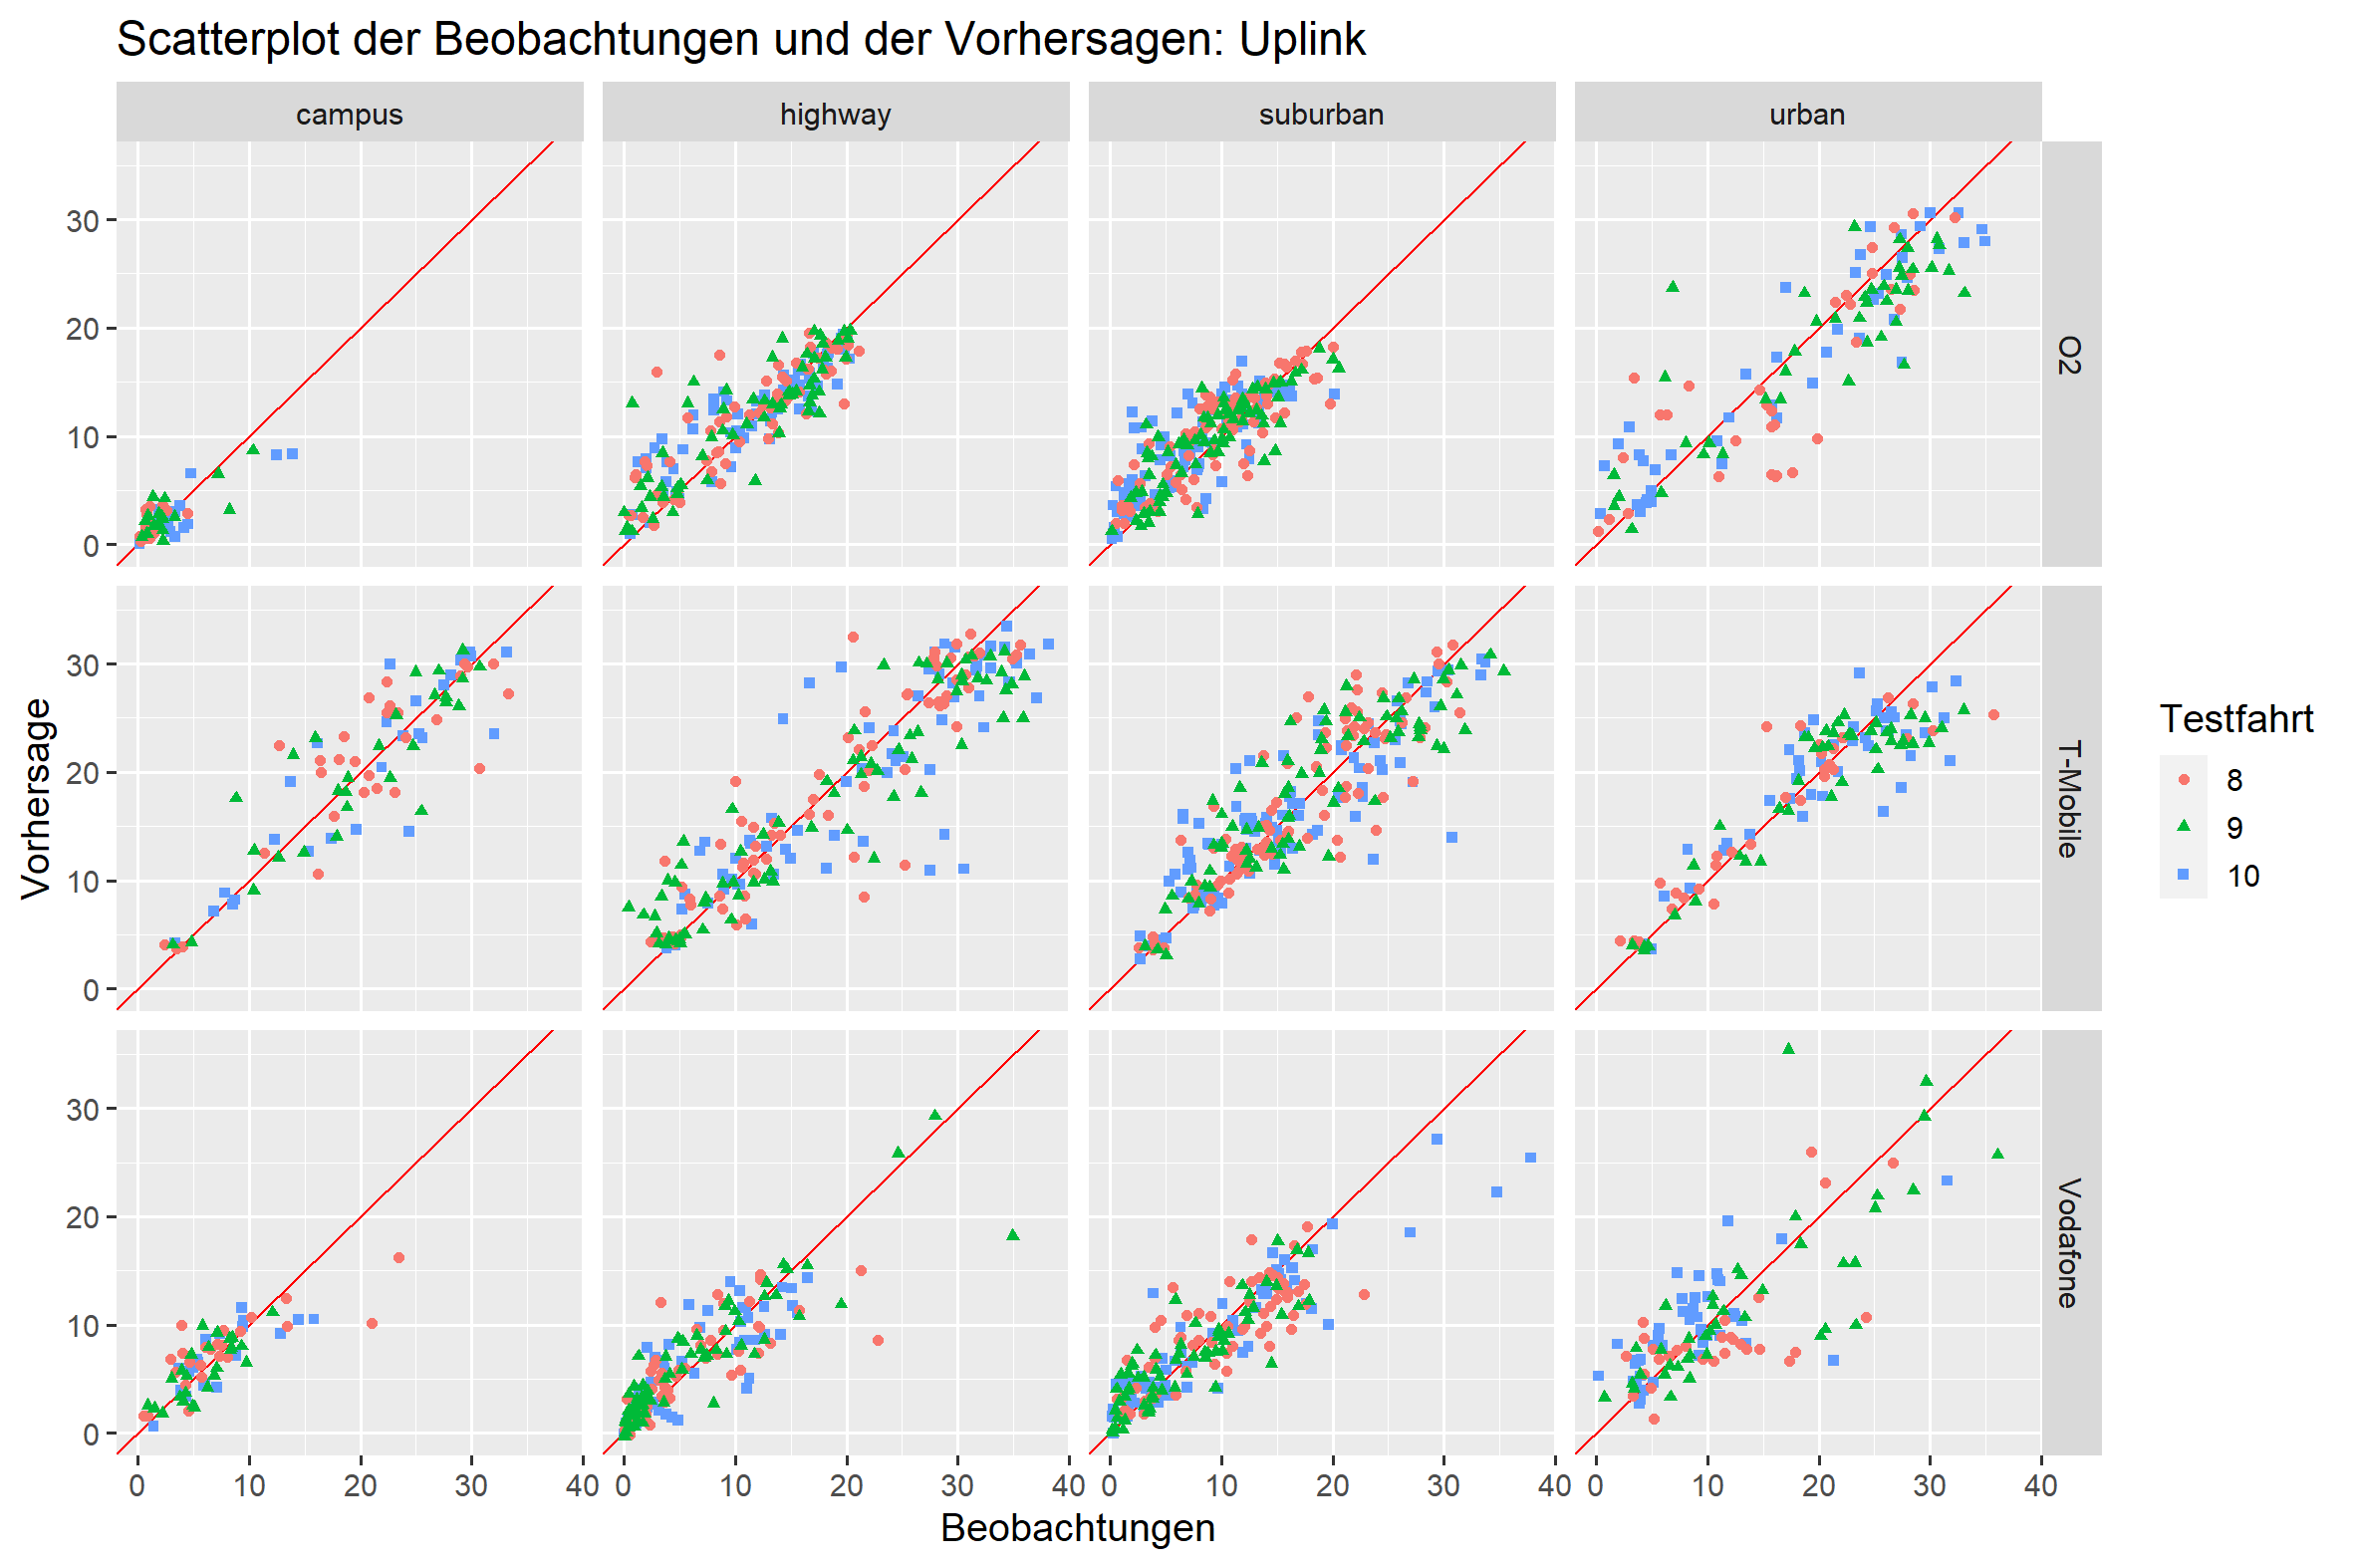
\includegraphics[width=\textwidth]{abbildungen/xgboost_predictions_ul}
\end{subfigure}
\begin{subfigure}{\textwidth}
    \centering
    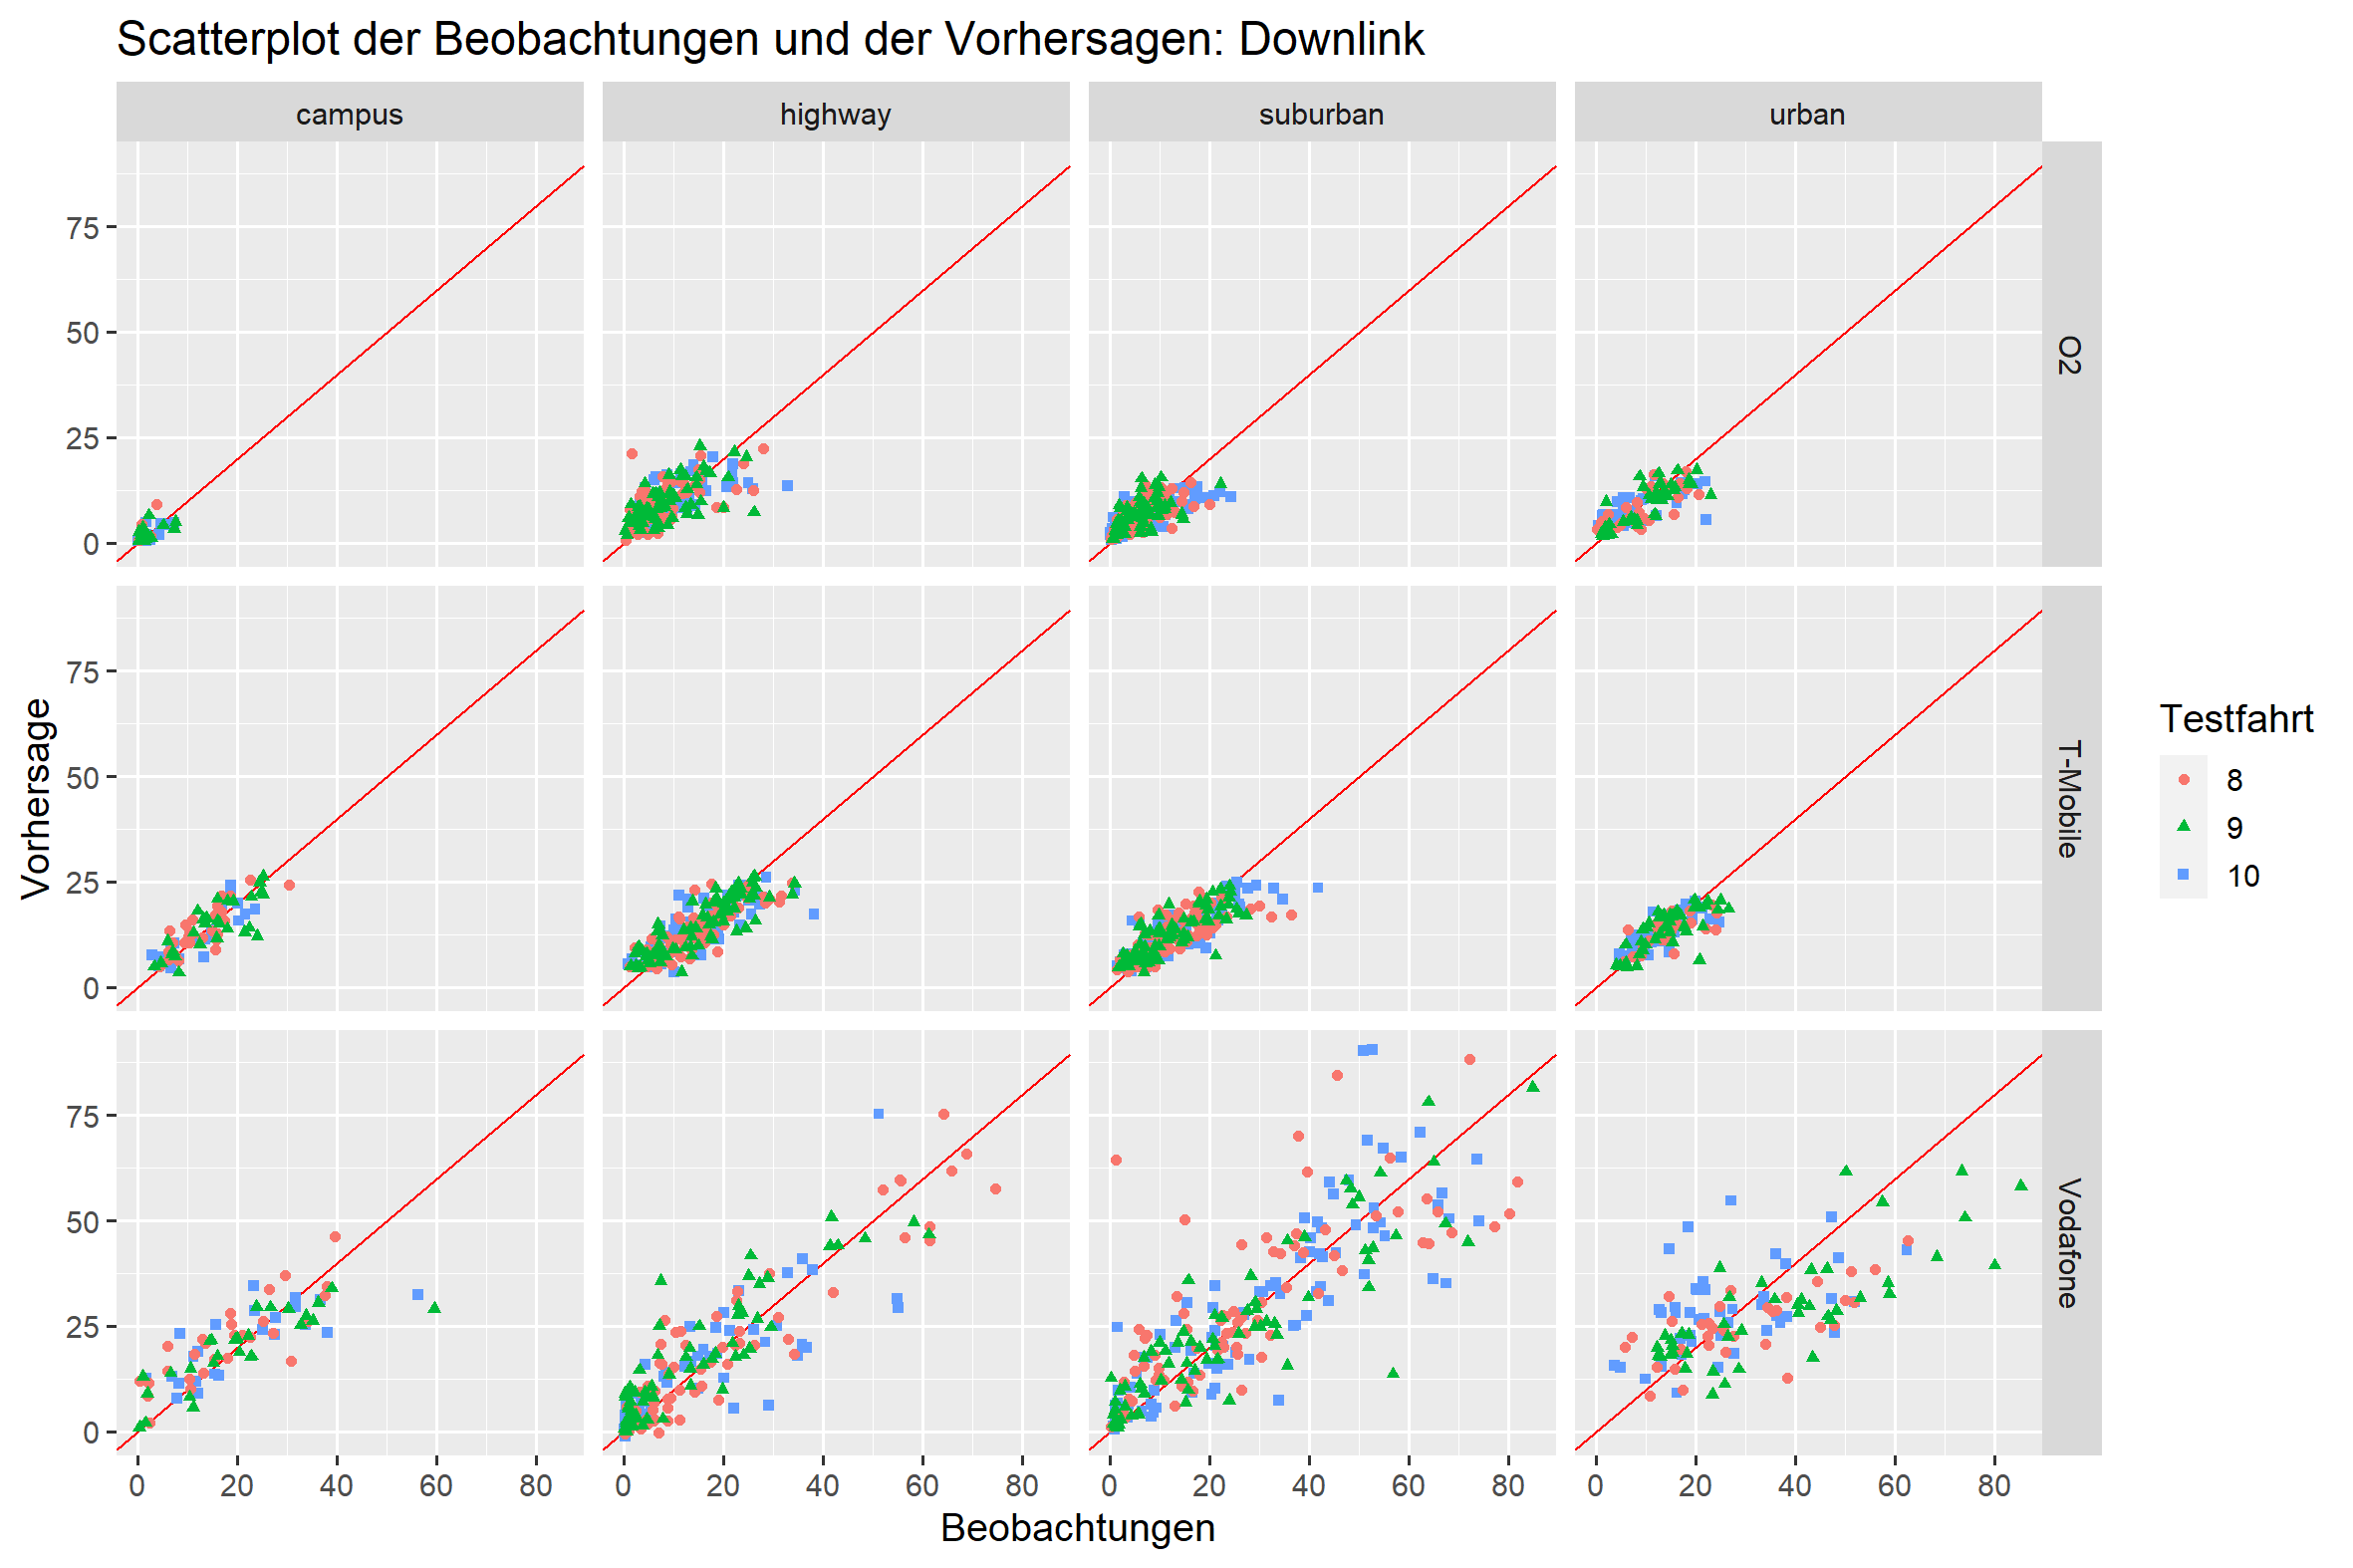
\includegraphics[width=\textwidth]{abbildungen/xgboost_predictions_dl}
\end{subfigure}
\caption{Out-of-Sample Vorhersagen der Datenraten f\"ur Extreme Gradient Boosting.}
\label{fig:datarate-predictions-xgboost}
\end{figure}

\subsubsection{Regression mit ARMA-Fehlern}

F\"ur die lineare Regression mit ARMA-Fehlern finden sich die Out-of-Sample Vorhersagen in Abbildung~\ref{fig:datarate-predictions-arma}.
Vergleicht man diese mit den Vorhersagen des Extreme Gradient Boosting, so fallen hier schon etwas st\"arkere systematische
Abweichungen ins Auge.
Beispielsweise scheint es so, dass im \textit{urban} Szenario f\"ur den Anbieter O2 h\"ohere Upload-Raten systematisch untersch\"atzt
und niedrigere Upload-Raten systematisch \"ubersch\"atzt werden.
Dies gibt einen ersten Aufschluss dar\"uber, dass das Modell m\"oglicherweise nicht ausdrucksstark genug sein k\"onnte,
um die Zusammenh\"ange in den Daten zu erfassen.
\begin{figure}
\centering
\begin{subfigure}{\textwidth}
    \centering
    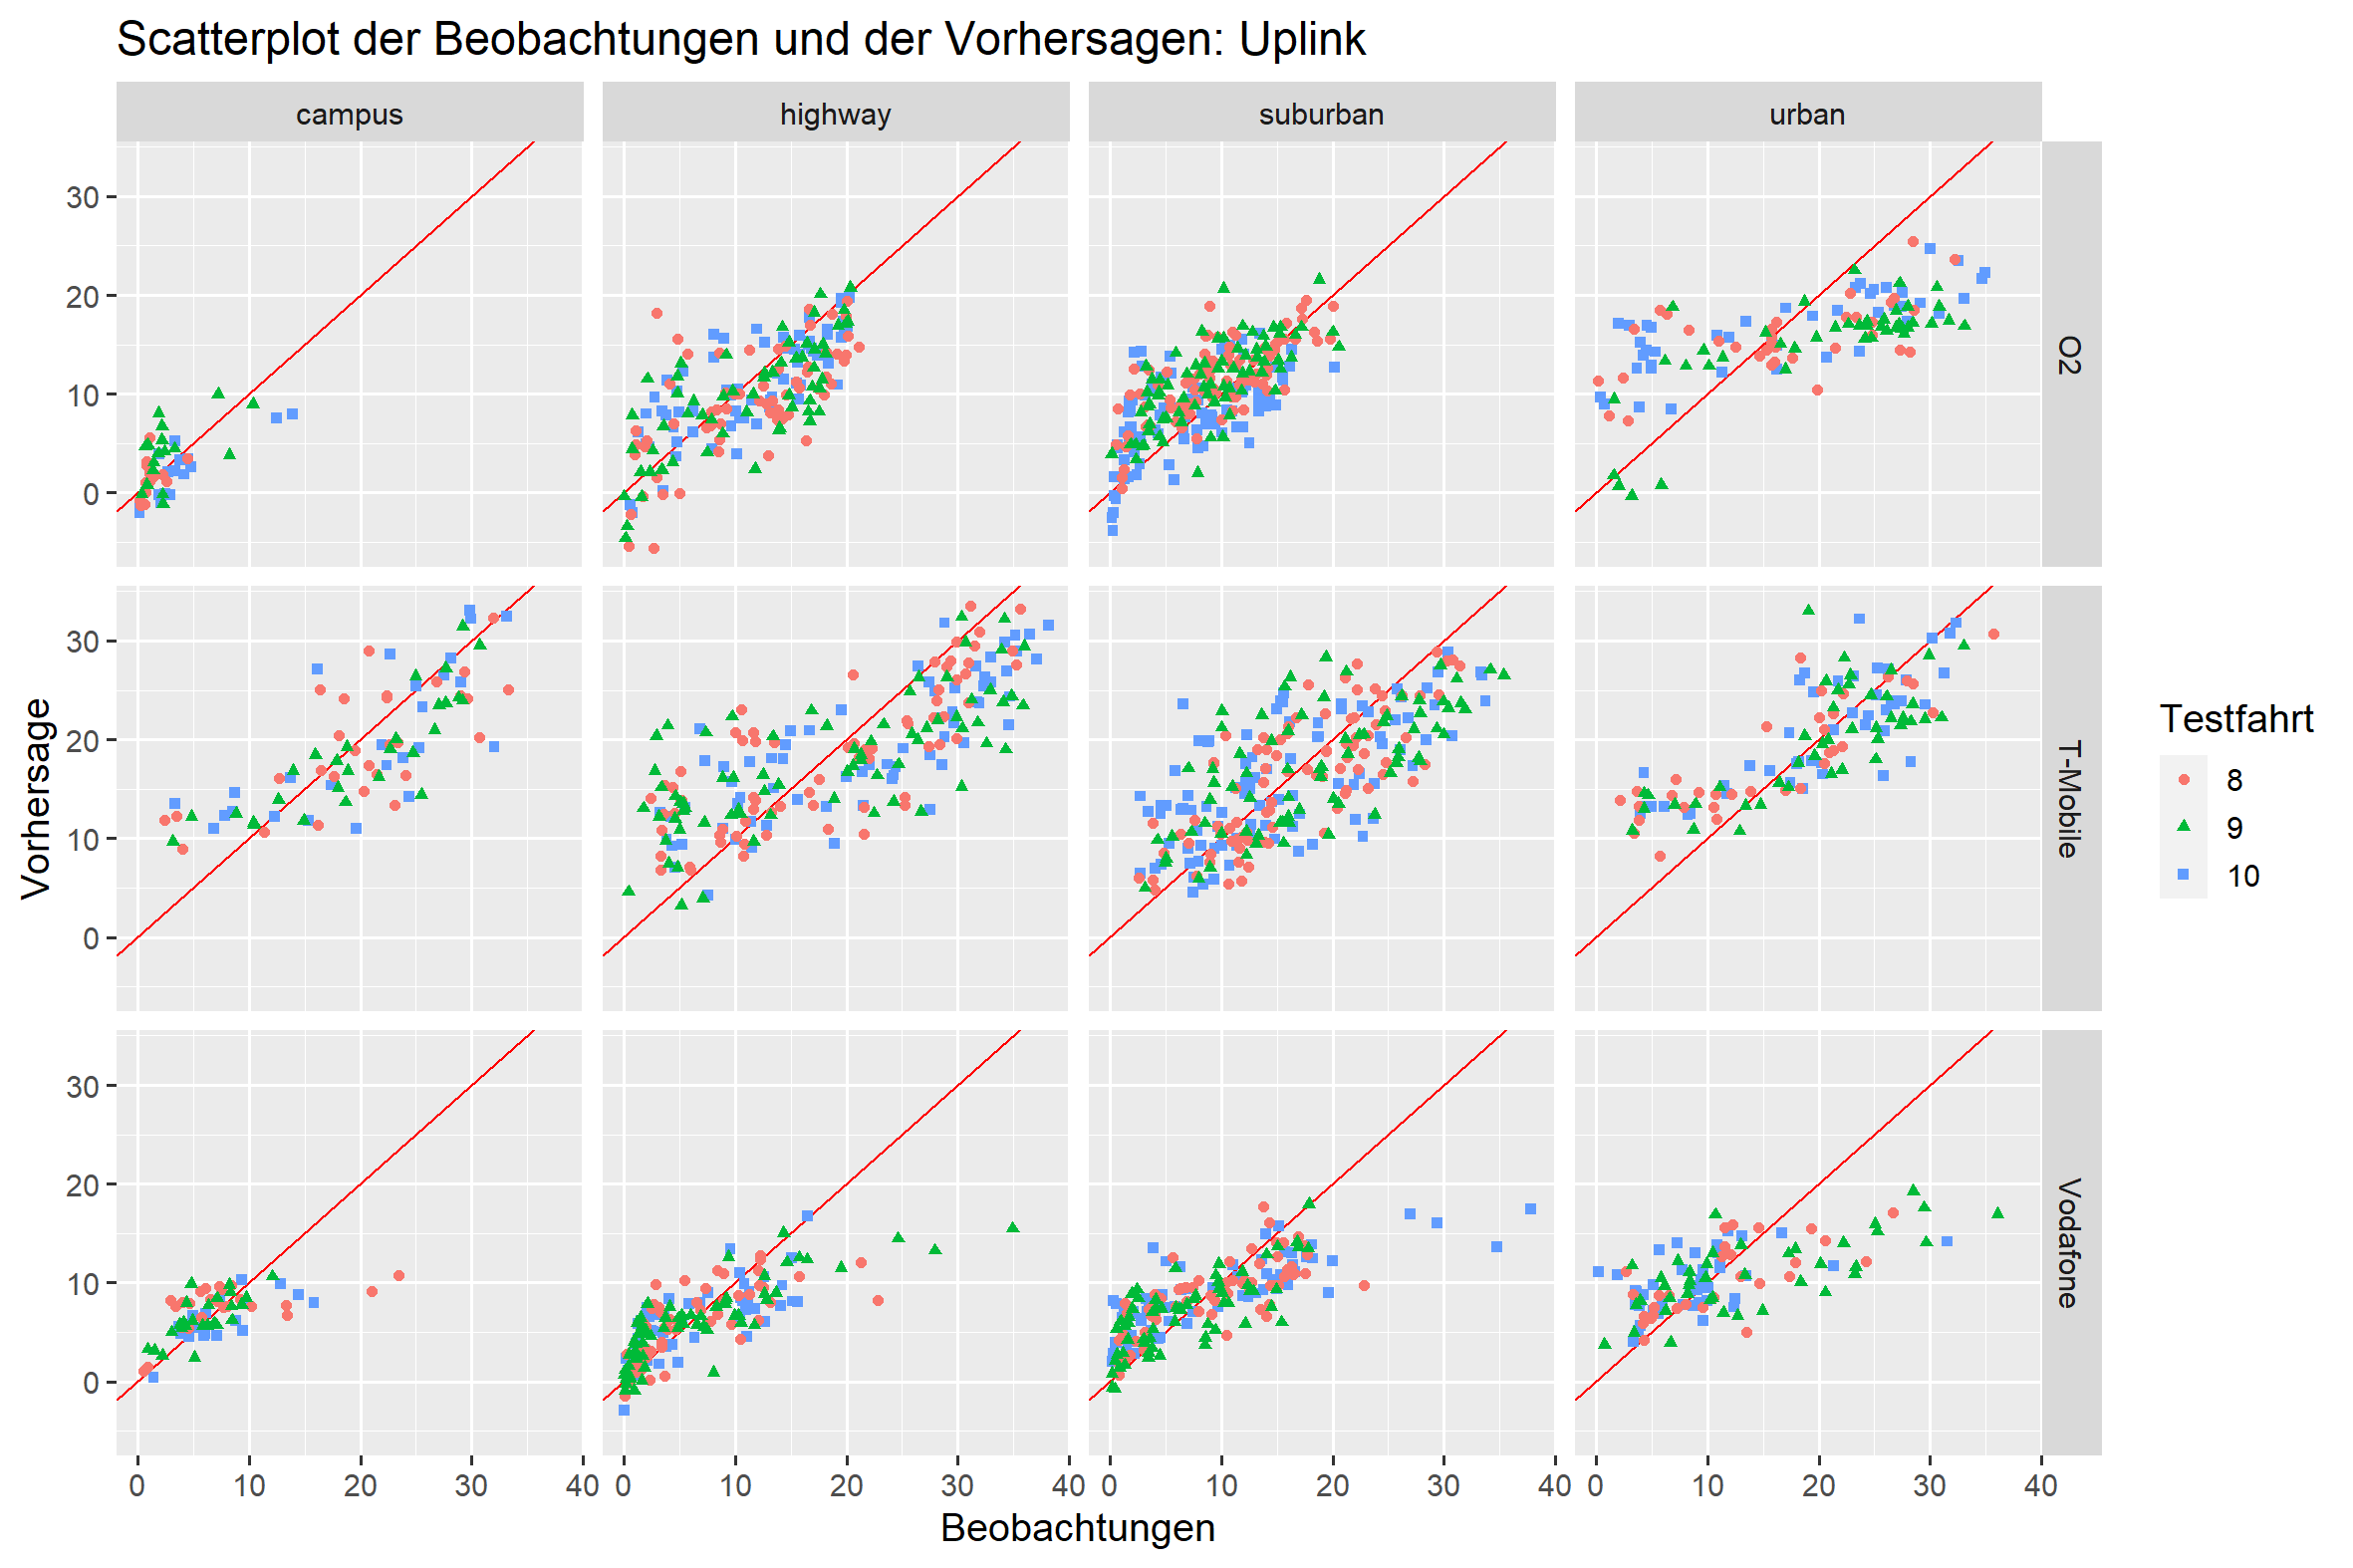
\includegraphics[width=\textwidth]{abbildungen/arma_predictions_ul}
\end{subfigure}
\begin{subfigure}{\textwidth}
    \centering
    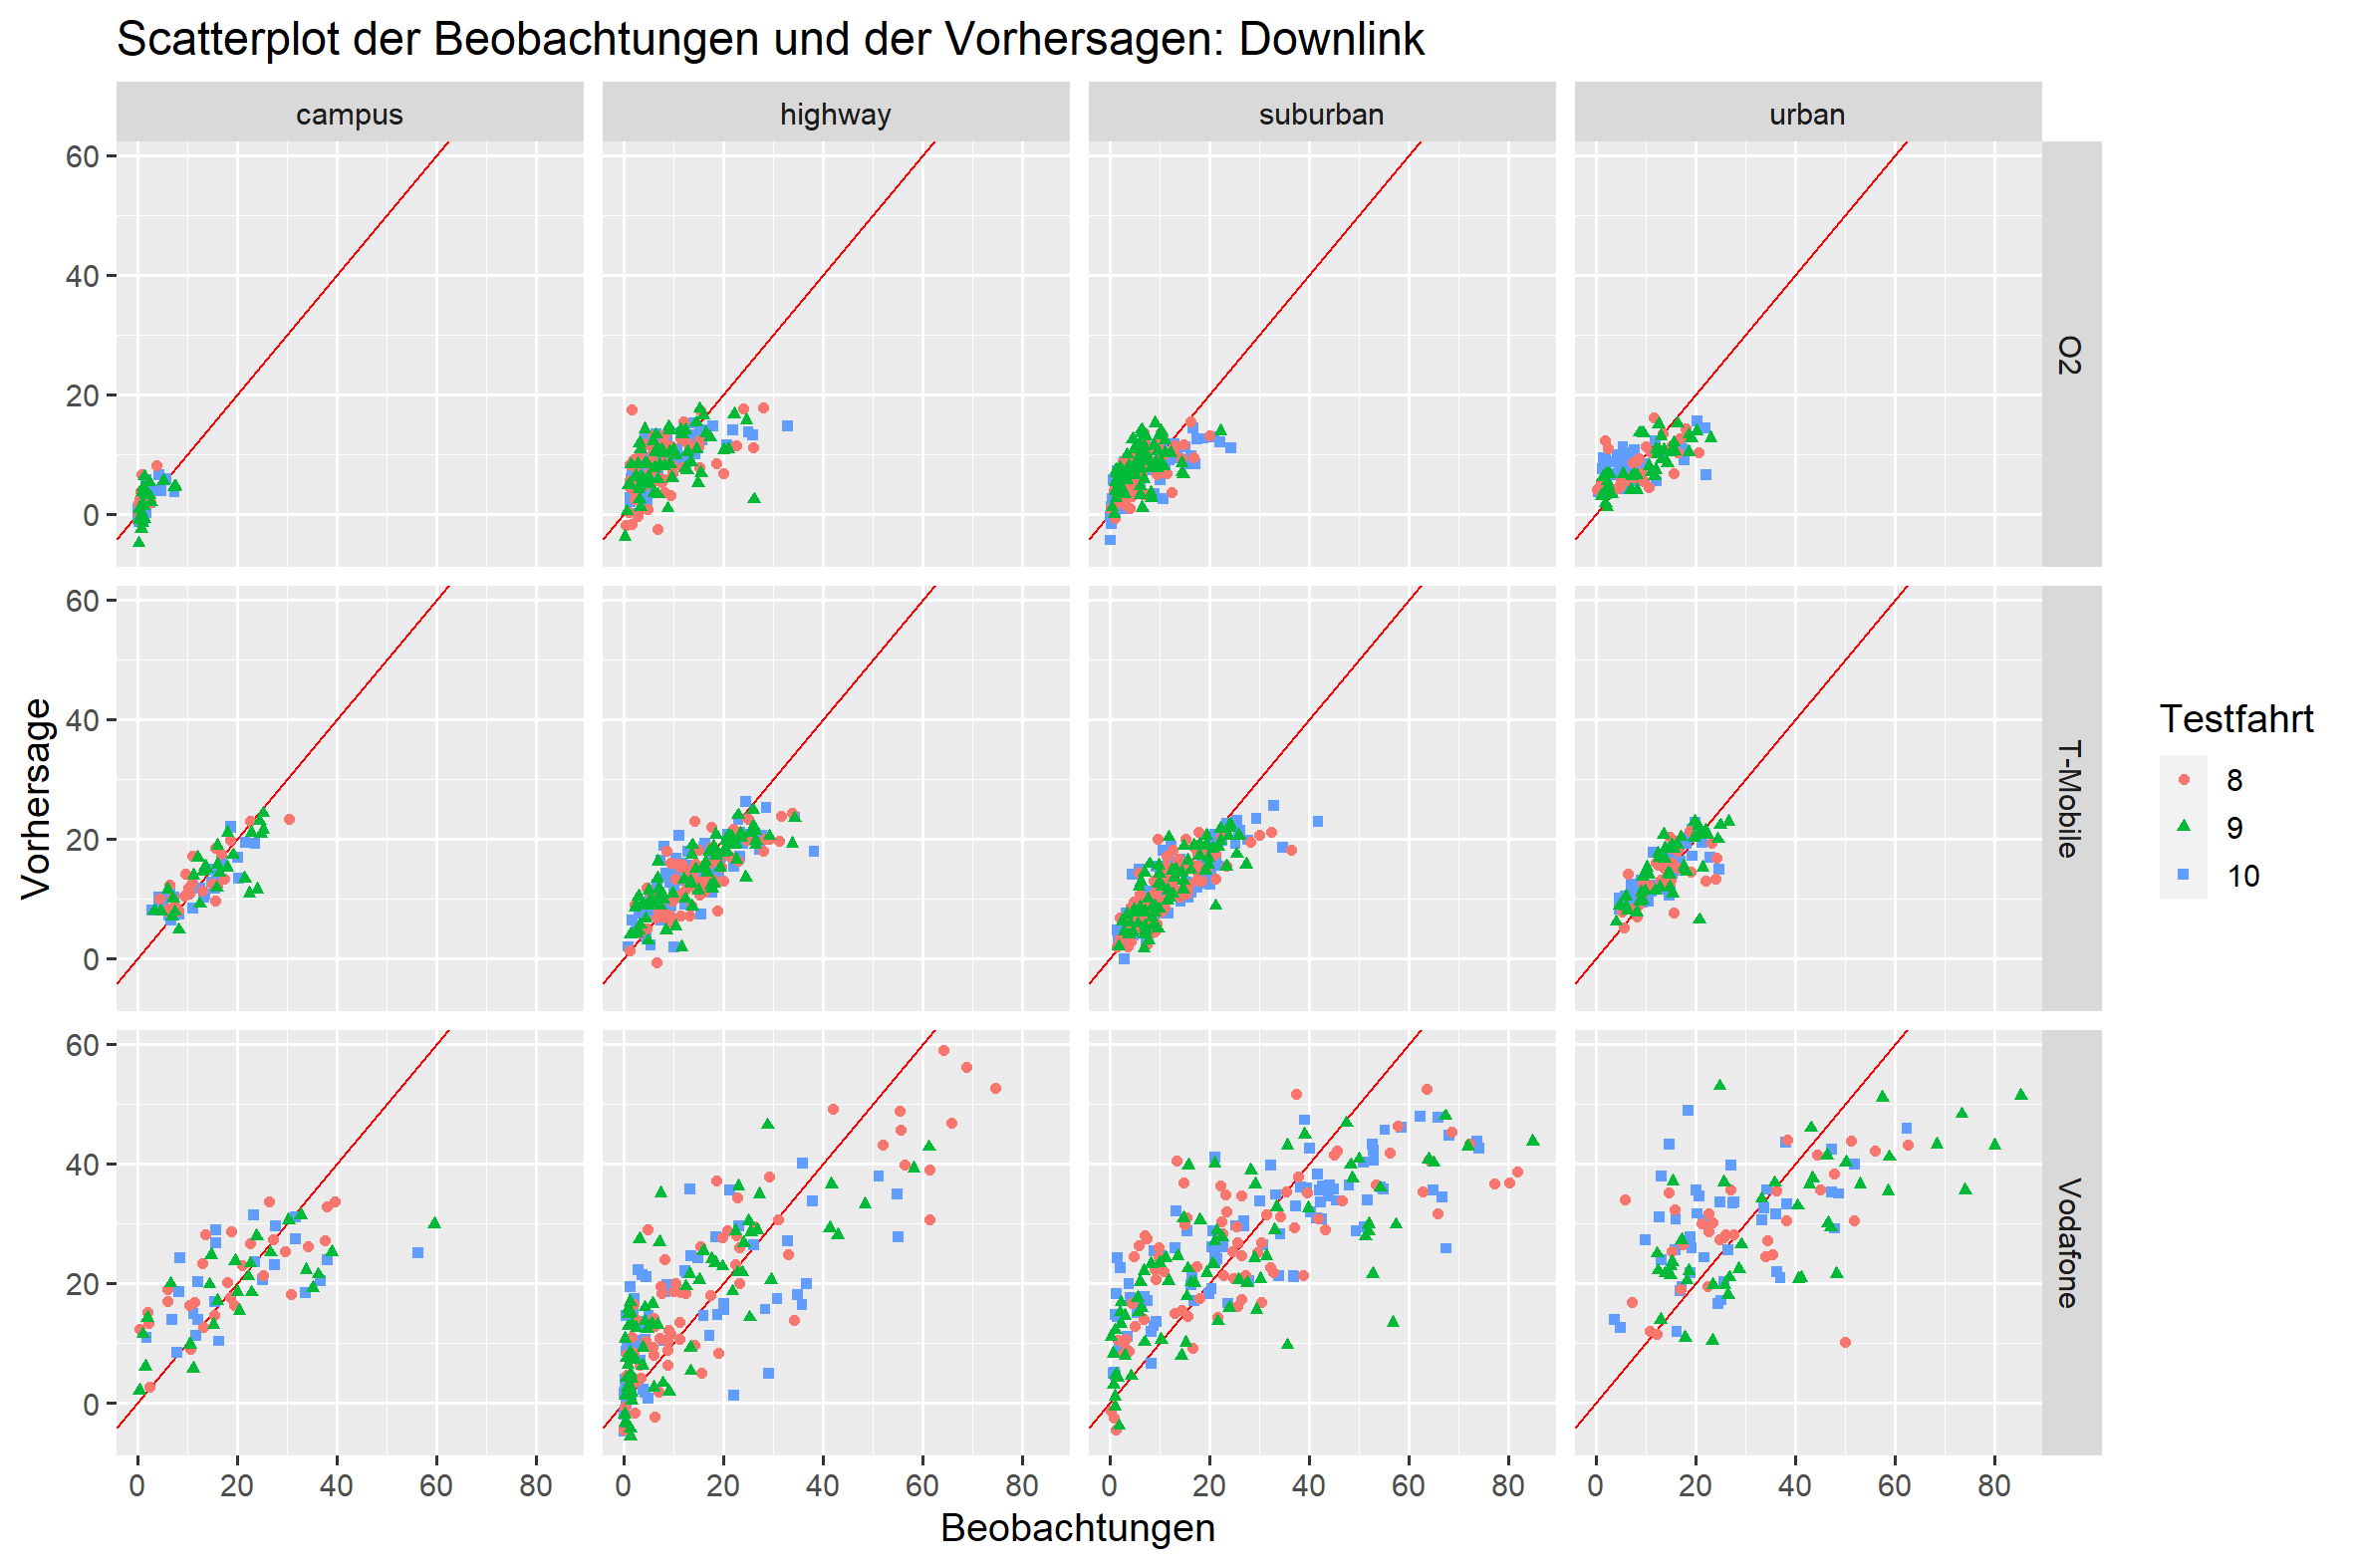
\includegraphics[width=\textwidth]{abbildungen/arma_predictions_dl}
\end{subfigure}
\caption{Out-of-Sample Vorhersagen der Datenraten f\"ur die Regression mit ARMA-Fehlern.}
\label{fig:datarate-predictions-arma}
\end{figure}

\subsubsection{Modellvergleich}

Die betrachteten Kennzahlen $R^2$ und $MAE$ wurden in Abbildung~\ref{fig:kennzahlen-datarate} einander gegen\"ubergestellt.
Man erkennt sofort, dass Extreme Gradient Boosting f\"ur jeden Anbieter die besseren Werte liefert, als die lineare Regression mit
ARMA-Fehlern.
Die Unterschiede sind hierbei allerdings je nach Art der Datenrate unterschiedlich hoch.
W\"ahrend das Extreme Gradient Boosting auf den Upload-Daten substantiell besser abschneidet,
so sind die Unterschiede auf den Download-Daten wesentlich geringer.

Bei den Download-Daten sticht noch der erh\"ohte Wert des MAE f\"ur den Anbieter Vodafone hervor.
Dieser ist jedoch vermutlich auf die h\"ohere Streuung in den Download-Raten dieses Providers zur\"uckzuf\"uhren und scheint die
Vorhersagequalit\"at der Modelle in diesem Fall nur begrenzt zu beschreiben, da das $R^2$ sowie die obigen Scatterplots
trotz des stark erh\"ohten MAE keine Verschlechterung bei der Vorhersagequalit\"at vermuten lassen.

Insgesamt l\"asst sich auf Basis dieser Kennzahlen sowie der Scatterplots der Out-of-Sample Vorhersagen erkennen, dass zumindest
davon ausgegangen werden kann, dass ein ausreichend starker Zusammenhang zwischen den Daten besteht, welcher eine Vorhersage
\"uberhaupt erst erm\"oglicht und sinnvoll macht.
Ob die erreichte Vorhersagequalit\"at aber f\"ur einen Einsatz in DDNS-Verfahren ausreichend ist,
m\"ussen nun die Anwender entscheiden.
\begin{figure}
\centering
\begin{subfigure}{0.49\textwidth}
    \centering
    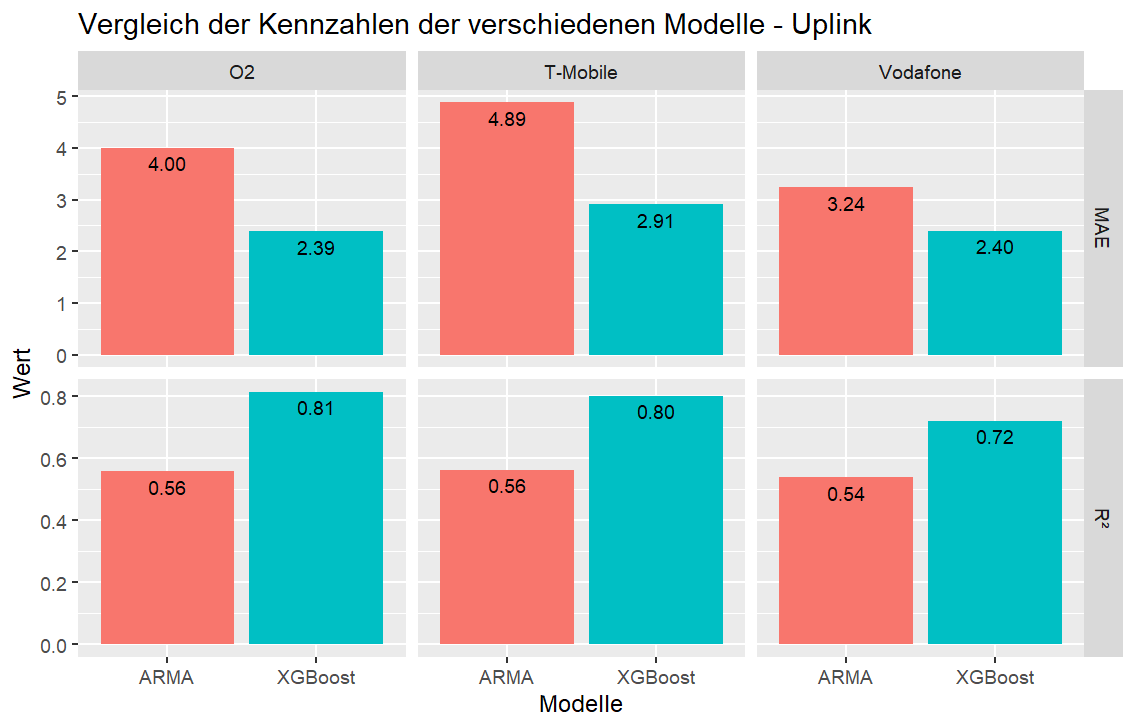
\includegraphics[width=\textwidth]{abbildungen/kennzahlen_vergleich_uplink}
\end{subfigure}
\begin{subfigure}{0.49\textwidth}
    \centering
    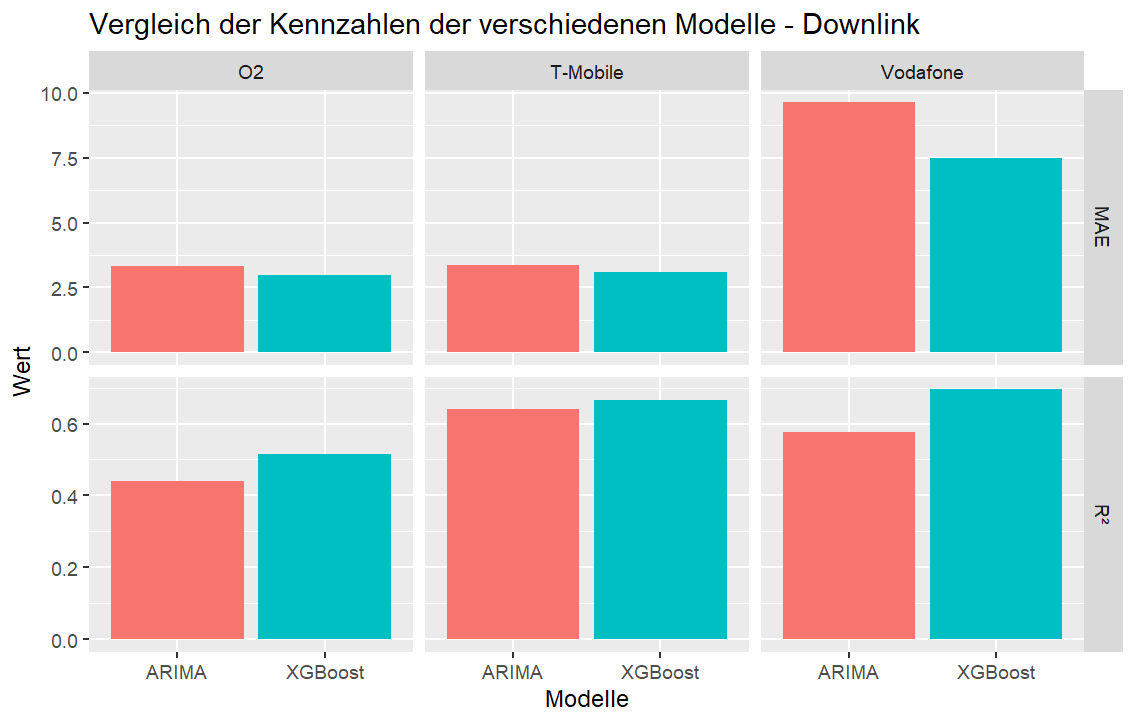
\includegraphics[width=\textwidth]{abbildungen/kennzahlen_vergleich_downlink}
\end{subfigure}
\caption{Vergleich der Kennzahlen f\"ur die Pr\"adiktion der Upload- und Download-Raten.}
\label{fig:kennzahlen-datarate}
\end{figure}

\subsubsection{Relevanz der Kovariablen}

Die Relevanz der einzelnen Kovariablen f\"ur die beiden Pr\"adiktionsmodelle wurde in Abbildung~\ref{fig:feature-importance-datenraten}
dargestellt.
Wie in Abschnitt~\ref{sec:xgboost-relevanz} beschrieben, wurden diese beim Extreme Gradient Boosting durch das
Permutation Feature Importance Verfahren ermittelt.
Bei der linearen Regression wurden hier die absoluten Gr\"o{\ss}en der Modellkoeffizienten berechnet, wobei die Daten zun\"achst
einheitlich skaliert wurden.
Beide Ma{\ss}e f\"ur die Relevanz der Kovariablen wurden anschlie{\ss}end zur besseren Vergleichbarkeit normiert.

Es f\"allt auf, dass die Variable Payload, also die Gr\"o{\ss}e des \"ubertragenen Datenpakets zur Messung der Daten\"ubertragungsrate,
f\"ur beide Modelle und sowohl f\"ur Download als auch Upload eine hohe Relevanz zu haben scheint.
Beim Extreme Gradient Boosting ist die Relevanz der Payload Variable sogar noch einmal deutlich st\"arker ausgepr\"agt, als bei
der Regression.
Wie sich der exakte Zusammenhang verh\"alt ist vermutlich ein Betriebsgeheimnis der Netzbetreiber, jedoch darf er vermutlich nicht
vernachl\"assigt werden.
Man sollte an dieser Stelle allerdings hinzuf\"ugen, dass Payload kein rein passiver Netzwerkindikator ist, sondern aktiv gemessen wurde.
Ob dies einen Einfluss auf die Einsatztauglichkeit der Modelle in DDNS haben k\"onnte, obliegt zur Entscheidung dem Anwender.
\begin{figure}
\centering
\begin{subfigure}{\textwidth}
    \centering
    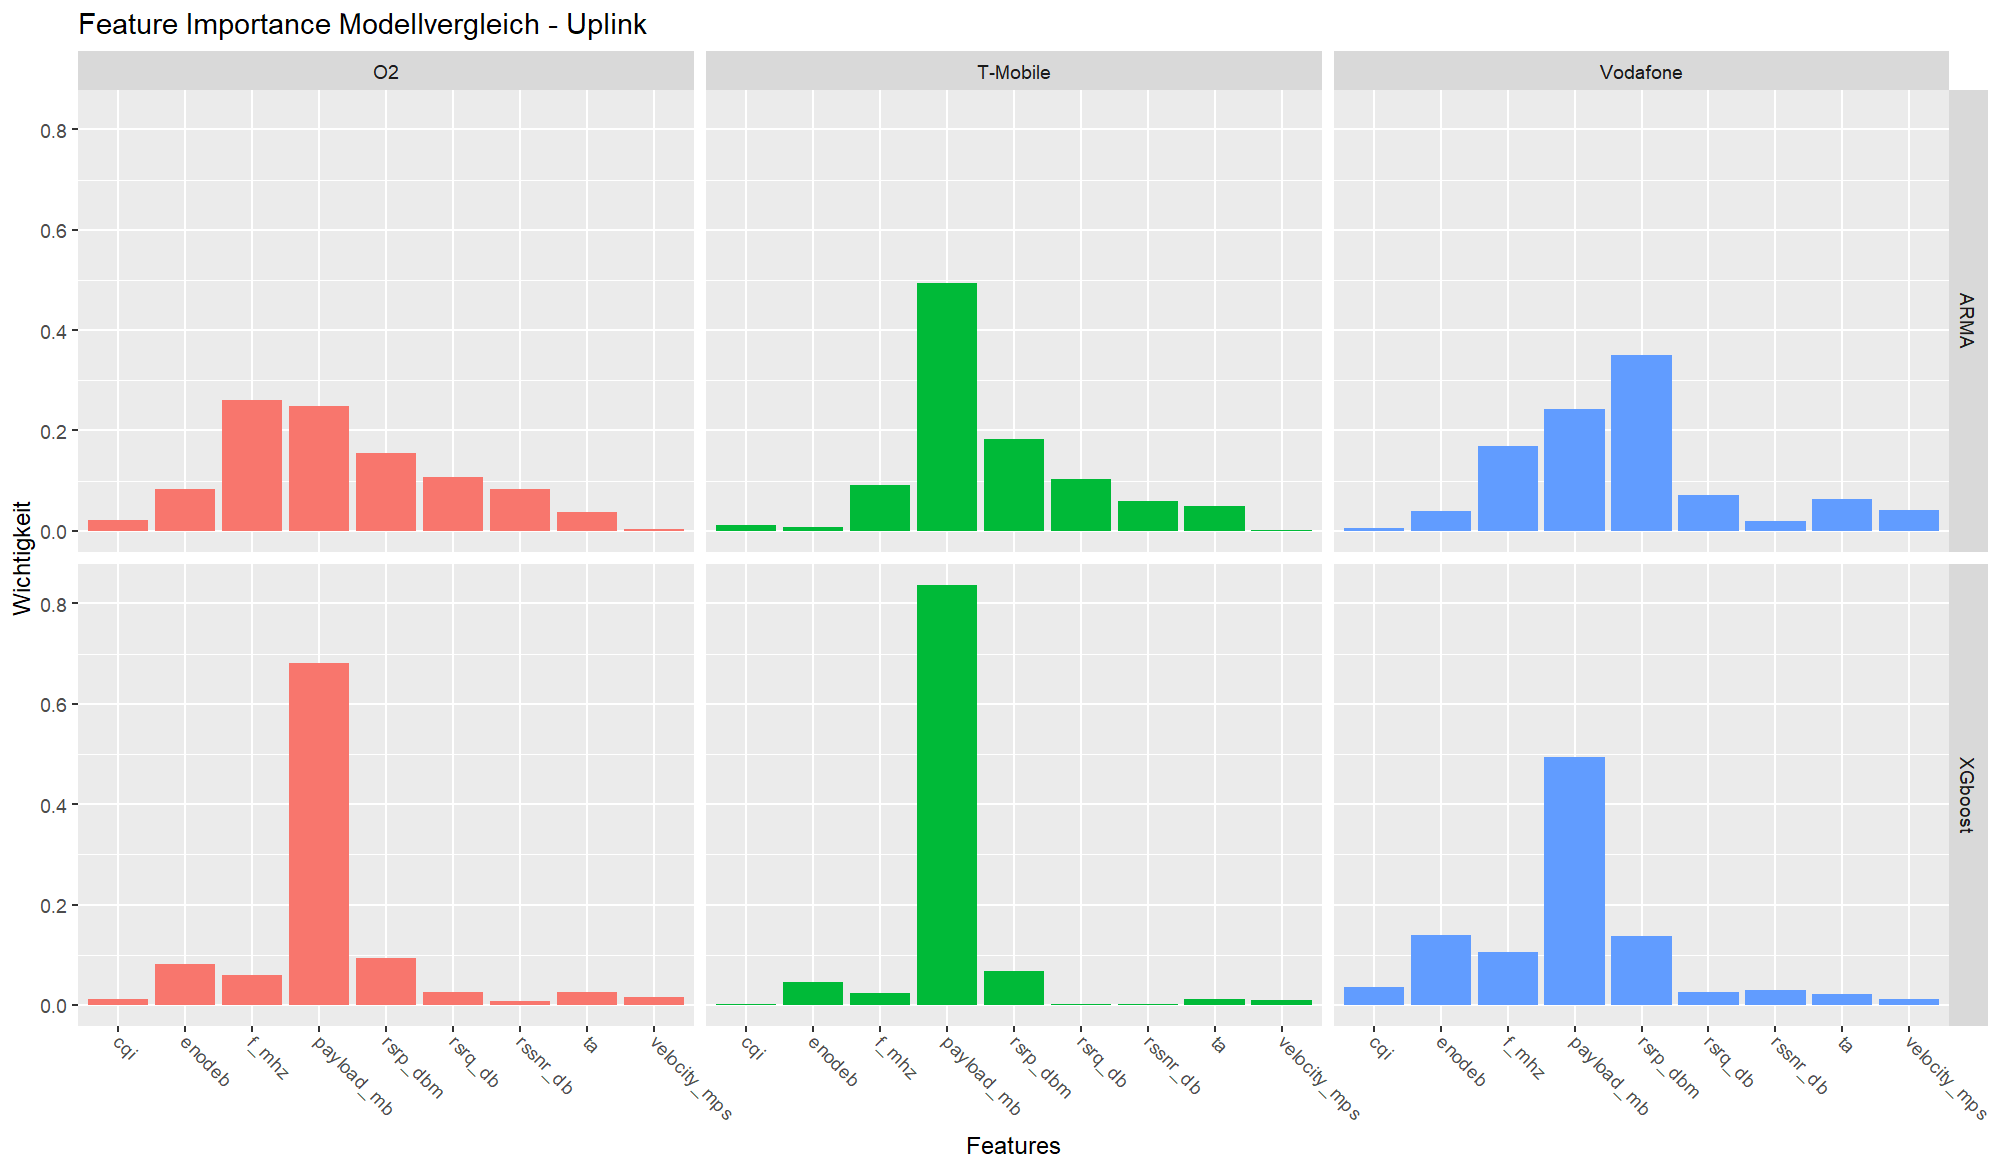
\includegraphics[width=\textwidth]{abbildungen/feature_importance_modellvergleich_uplink}
\end{subfigure}
\begin{subfigure}{\textwidth}
    \centering
    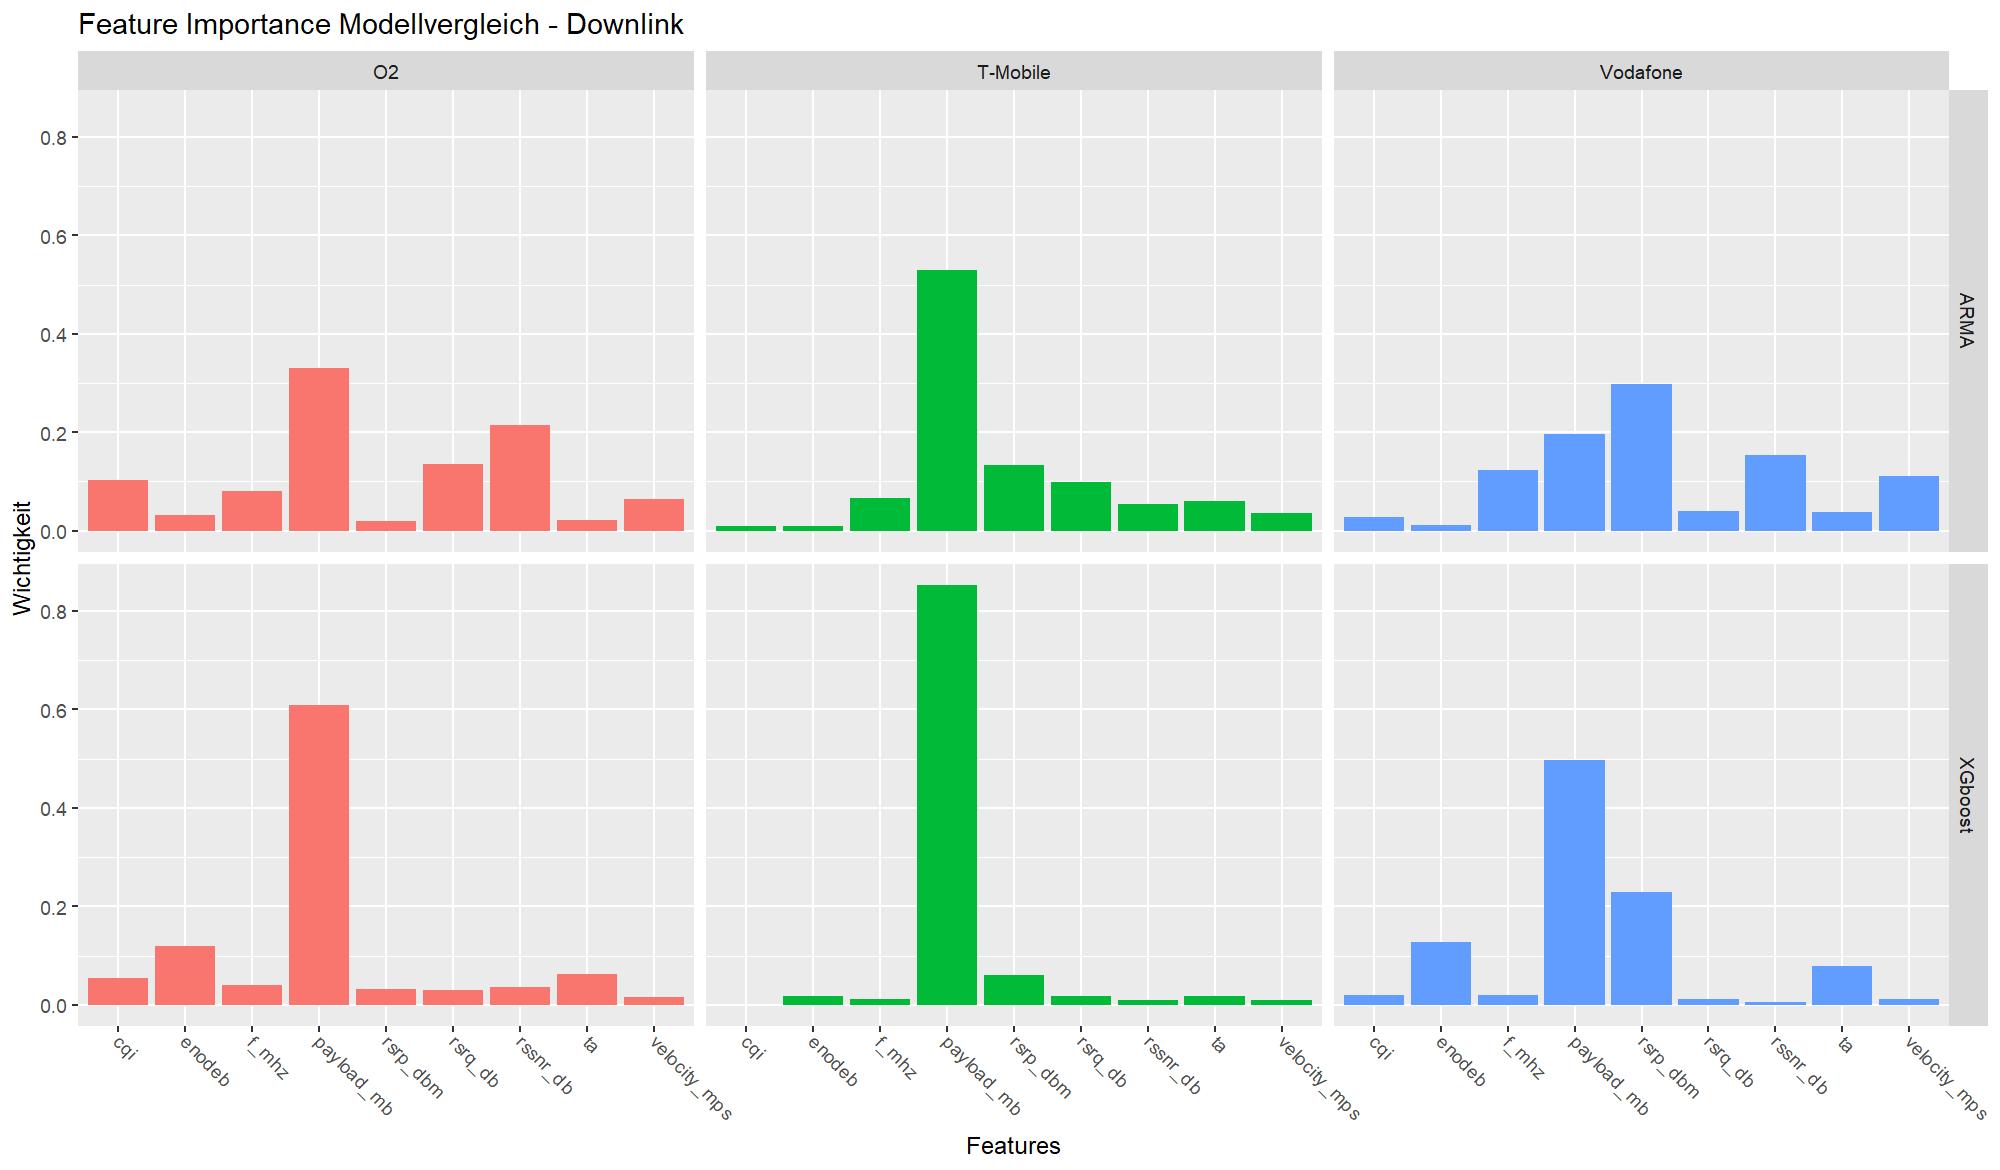
\includegraphics[width=\textwidth]{abbildungen/feature_importance_modellvergleich_downlink}
\end{subfigure}
\caption{Relevanz der Kovariablen bez\"uglich der beiden Modelle zur Datenratenpr\"adiktion.}
\label{fig:feature-importance-datenraten}
\end{figure}

\subsection{Vorhersage der eNodeB-Verbindungsdauern}

Die Vorhersage der eNodeB-Verbindungsdauern wurde analog zur Vorhersage der Daten\"ubertragungsraten durchgef\"uhrt.
Auch hier wurde das eingesetzte Vorhersagemodell, also das Extreme Gradient Boosting, zun\"achst wie in
Abschnitt~\ref{sec:validierung-tuning} beschrieben auf den Fahrten \mbox{1-7} trainiert und getuned und im Anschluss
auf den neuen und ungesehenen Daten der Fahrten \mbox{8-10} getestet.
Es wurde hier ebenfalls f\"ur jeden der Netzbetreiber ein eigenes Modell angepasst, 
die Out-of-Sample Vorhersagen finden sich in Abbildung~\ref{fig:link-lifetime-predictions}.
\begin{figure}
    \centering
    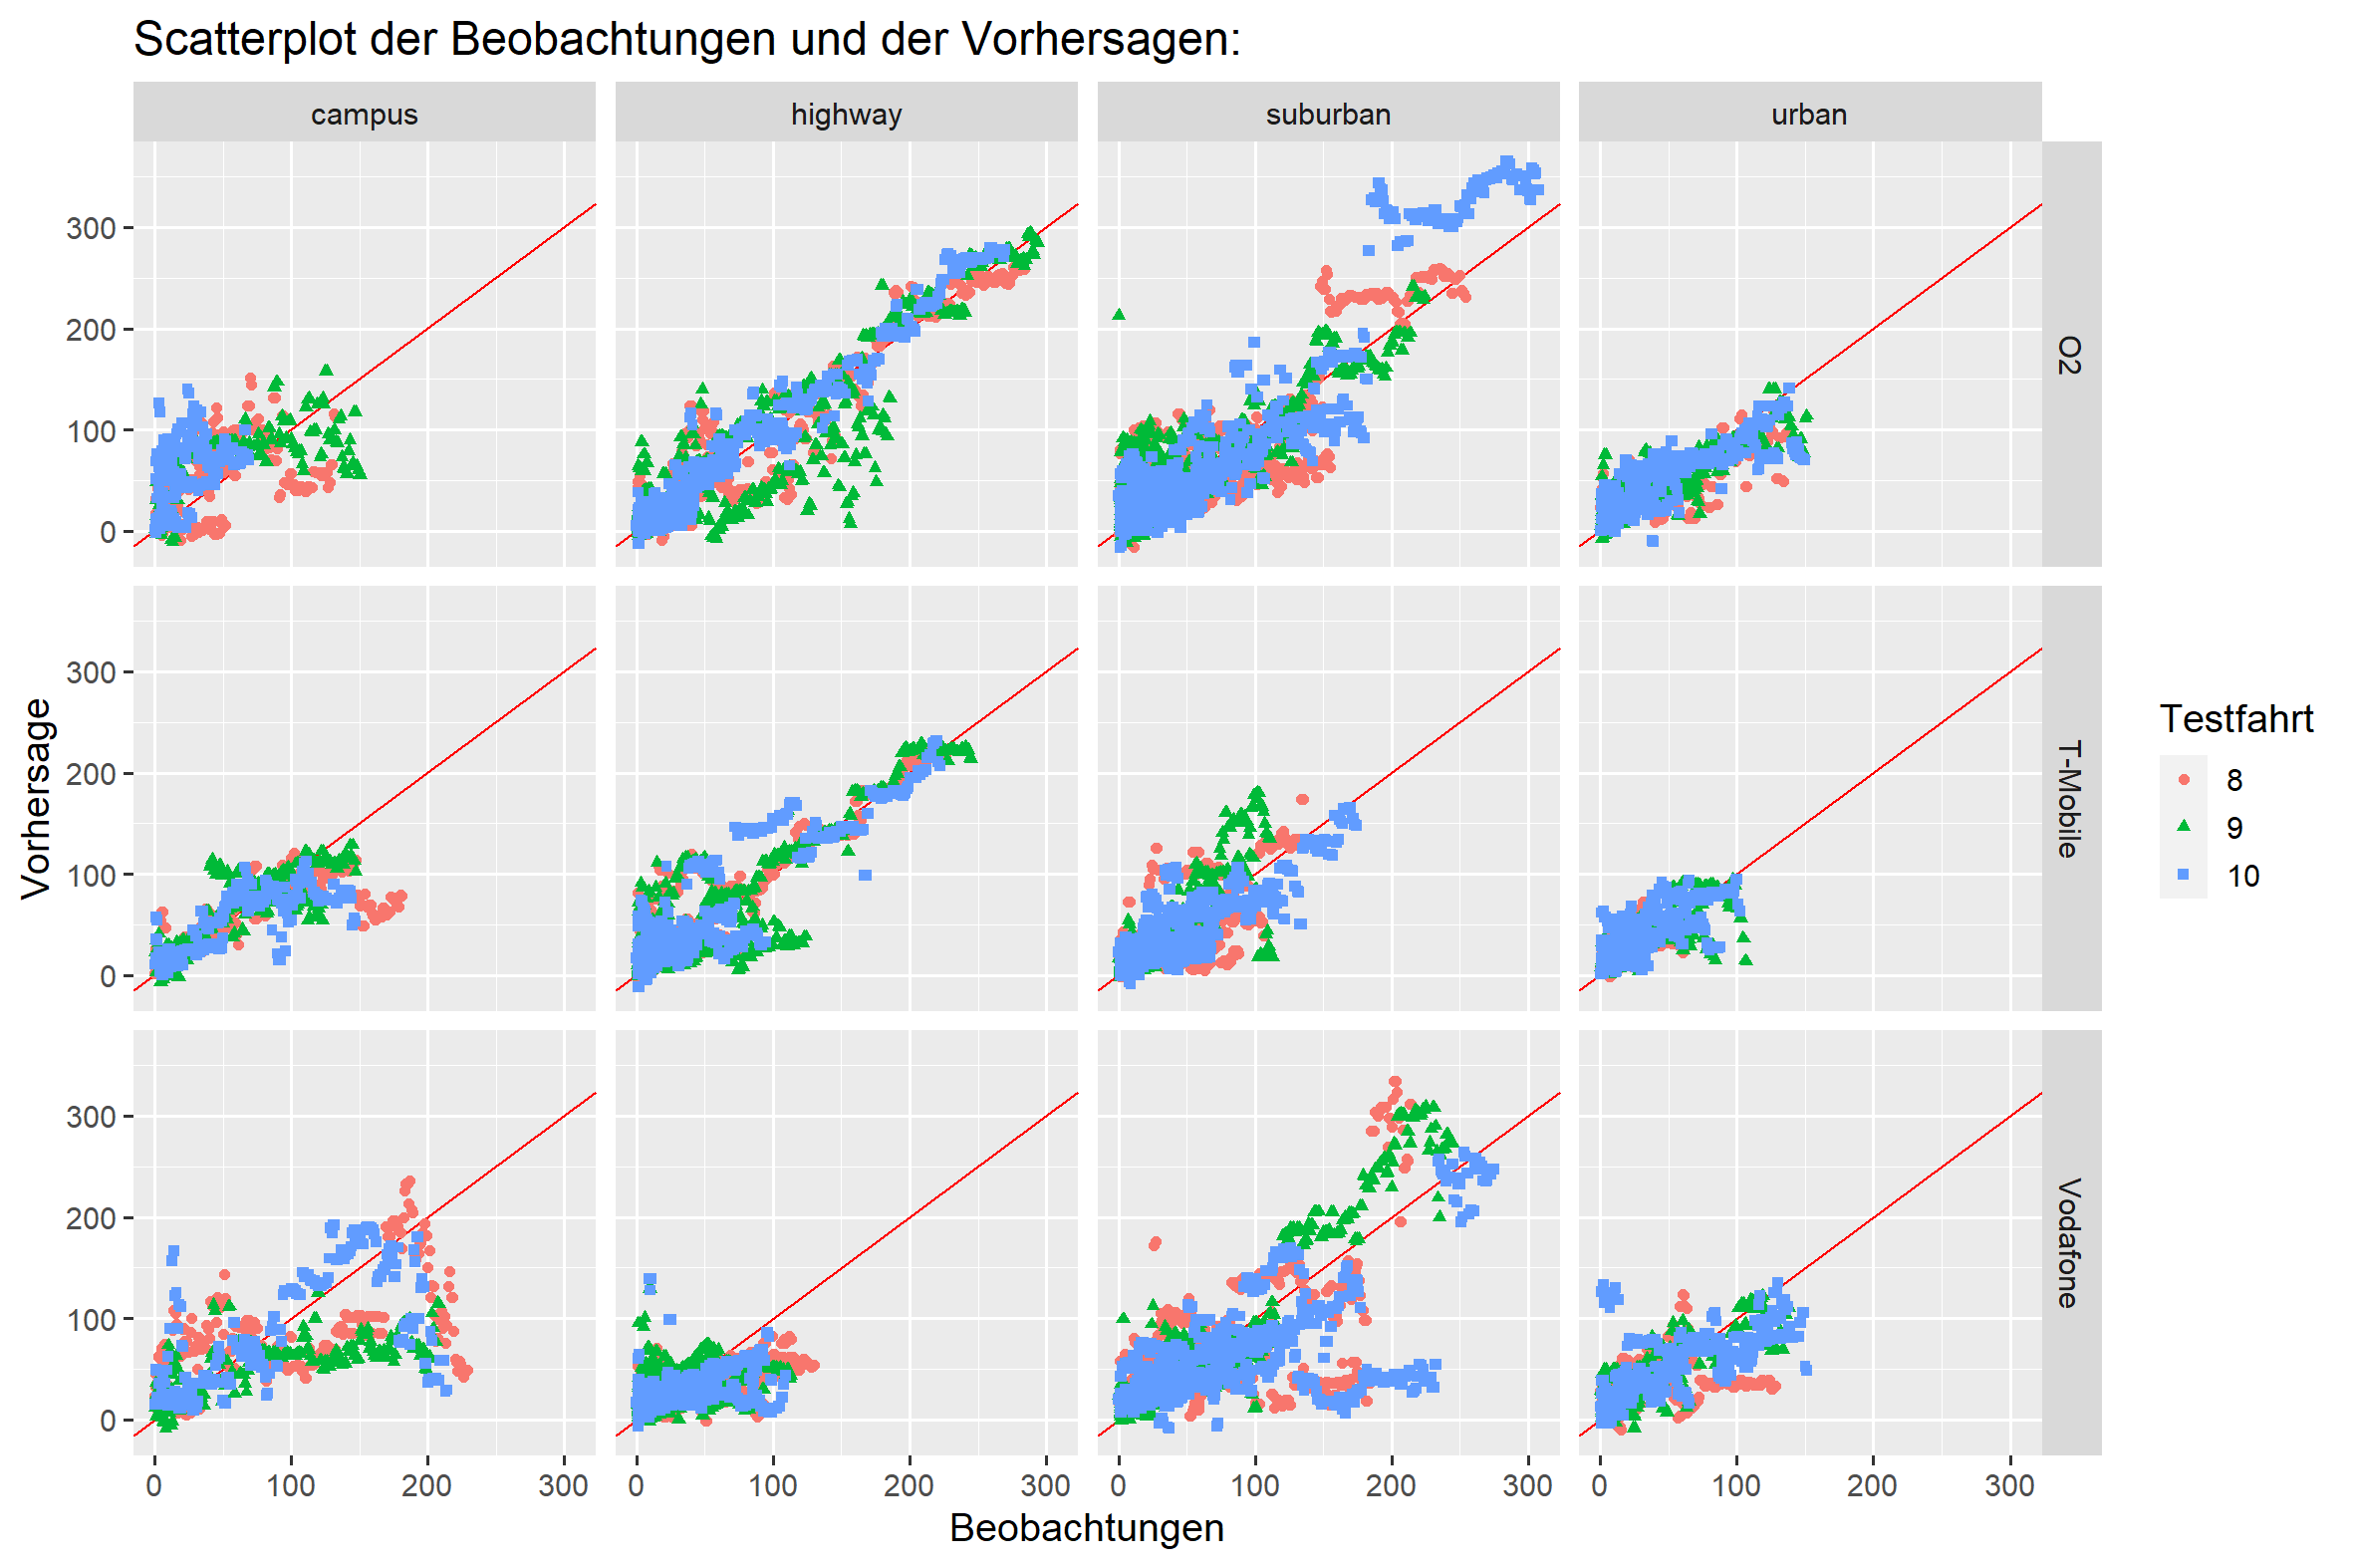
\includegraphics[width=\textwidth]{abbildungen/predictions_linklifetime}
    \caption{Out-of-Sample Vorhersagen der eNodeB-Verbindungsdauern.}
    \label{fig:link-lifetime-predictions}
\end{figure}
Anders als bei der Vorhersage der Datenraten lassen die Scatterplots hier schon erste Unregelm\"a{\ss}igkeiten erkennen.
Die Vorhersagepunkte streuen nicht sehr gleichm\"a{\ss}ig um die Winkelhalbierende, was auf systematische Modellfehler schlie{\ss}en
l\"asst.

Die Kennnzahlen des Modells sind in Abbildung~\ref{fig:kennzahlen-link-lifetime} gegeben.
Hier lassen sich Unterschiede zwischen den Anbietern feststellen. F\"ur den Provider Vodafone scheint das Modell nach beiden
Kriterien am schlechtesten abzuschneiden. O2 liefert das beste $R^2$ und T-Mobile den besten $MAE$.
Diese Unterschiede lassen sich vermutlich darauf zur\"uckf\"uhren, dass der Mechanismus des Funkmastwechsels bei den verschiedenen
Anbietern unterschiedlich realisiert wurde.
\begin{figure}
    \centering
    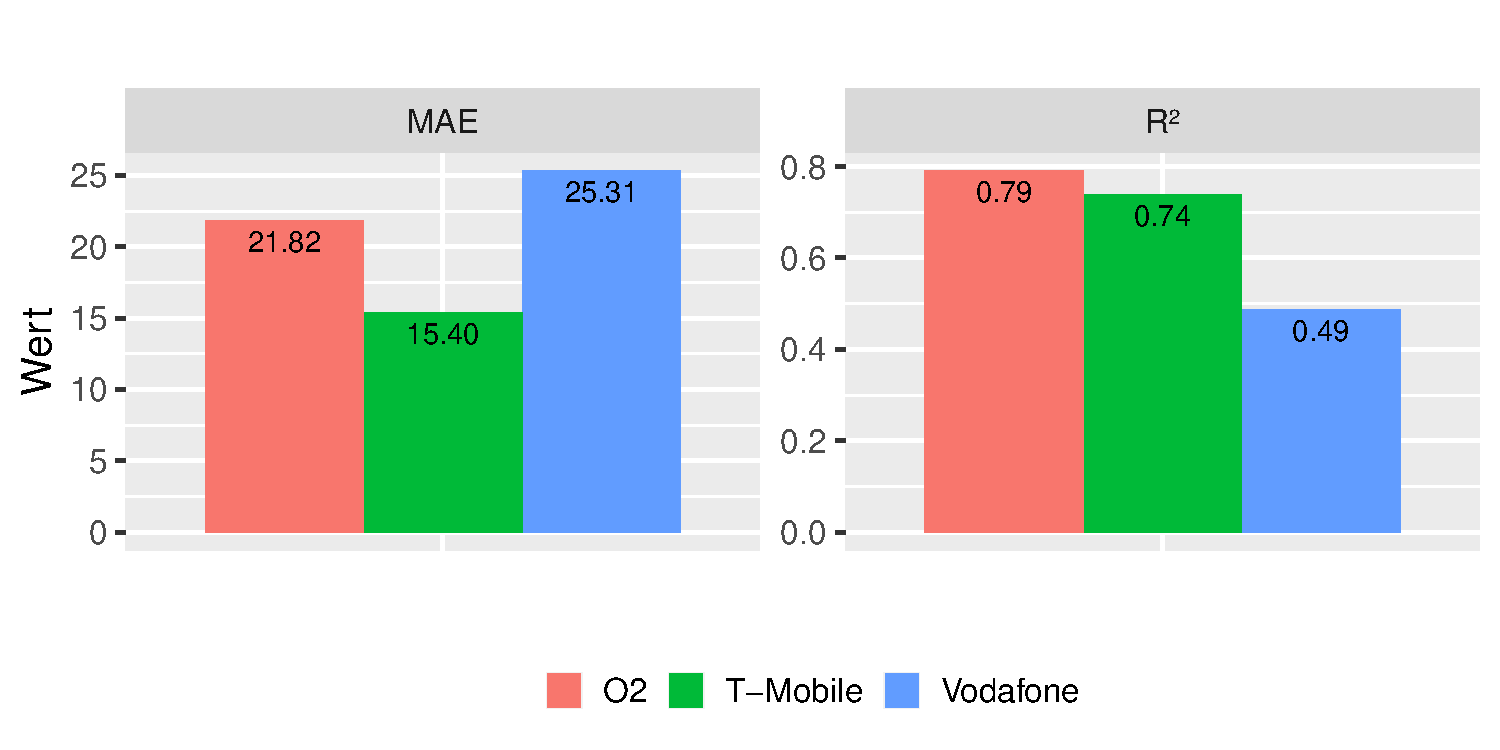
\includegraphics[width=0.6\textwidth]{abbildungen/kennzahlen_linklifetime}
    \caption{Kennzahlen Link-Lifetime Vorhersage des Extreme Gradient Boosting.}
    \label{fig:kennzahlen-link-lifetime}
\end{figure}

Um zu zeigen, wie sich diese Unterschiede auswirken k\"onnen, sind in Abbildung~\ref{fig:link-lifetime-zeitreihe} die Out-of-Sample
Vorhersagen der eNodeB-Verbindungsdauern f\"ur die Anbieter O2 und Vodafone einmal als Zeitreihe dargestellt.
Man erkennt zwar insbesondere beim besser abschneidenden O2 Modell, dass die Vorhersagen teilweise schon mit den Beobachtungen
einhergehen, jedoch sind die Streuungen und Abweichungen bei beiden Modellen teilweise sehr stark ausgepr\"agt.
Es ist also wirklich fraglich und bleibt zu \"uberpr\"ufen, ob diese Vorhersagen einen brauchbaren Mehrwert liefern k\"onnen.
\begin{figure}
\centering
\begin{subfigure}{\textwidth}
    \centering
    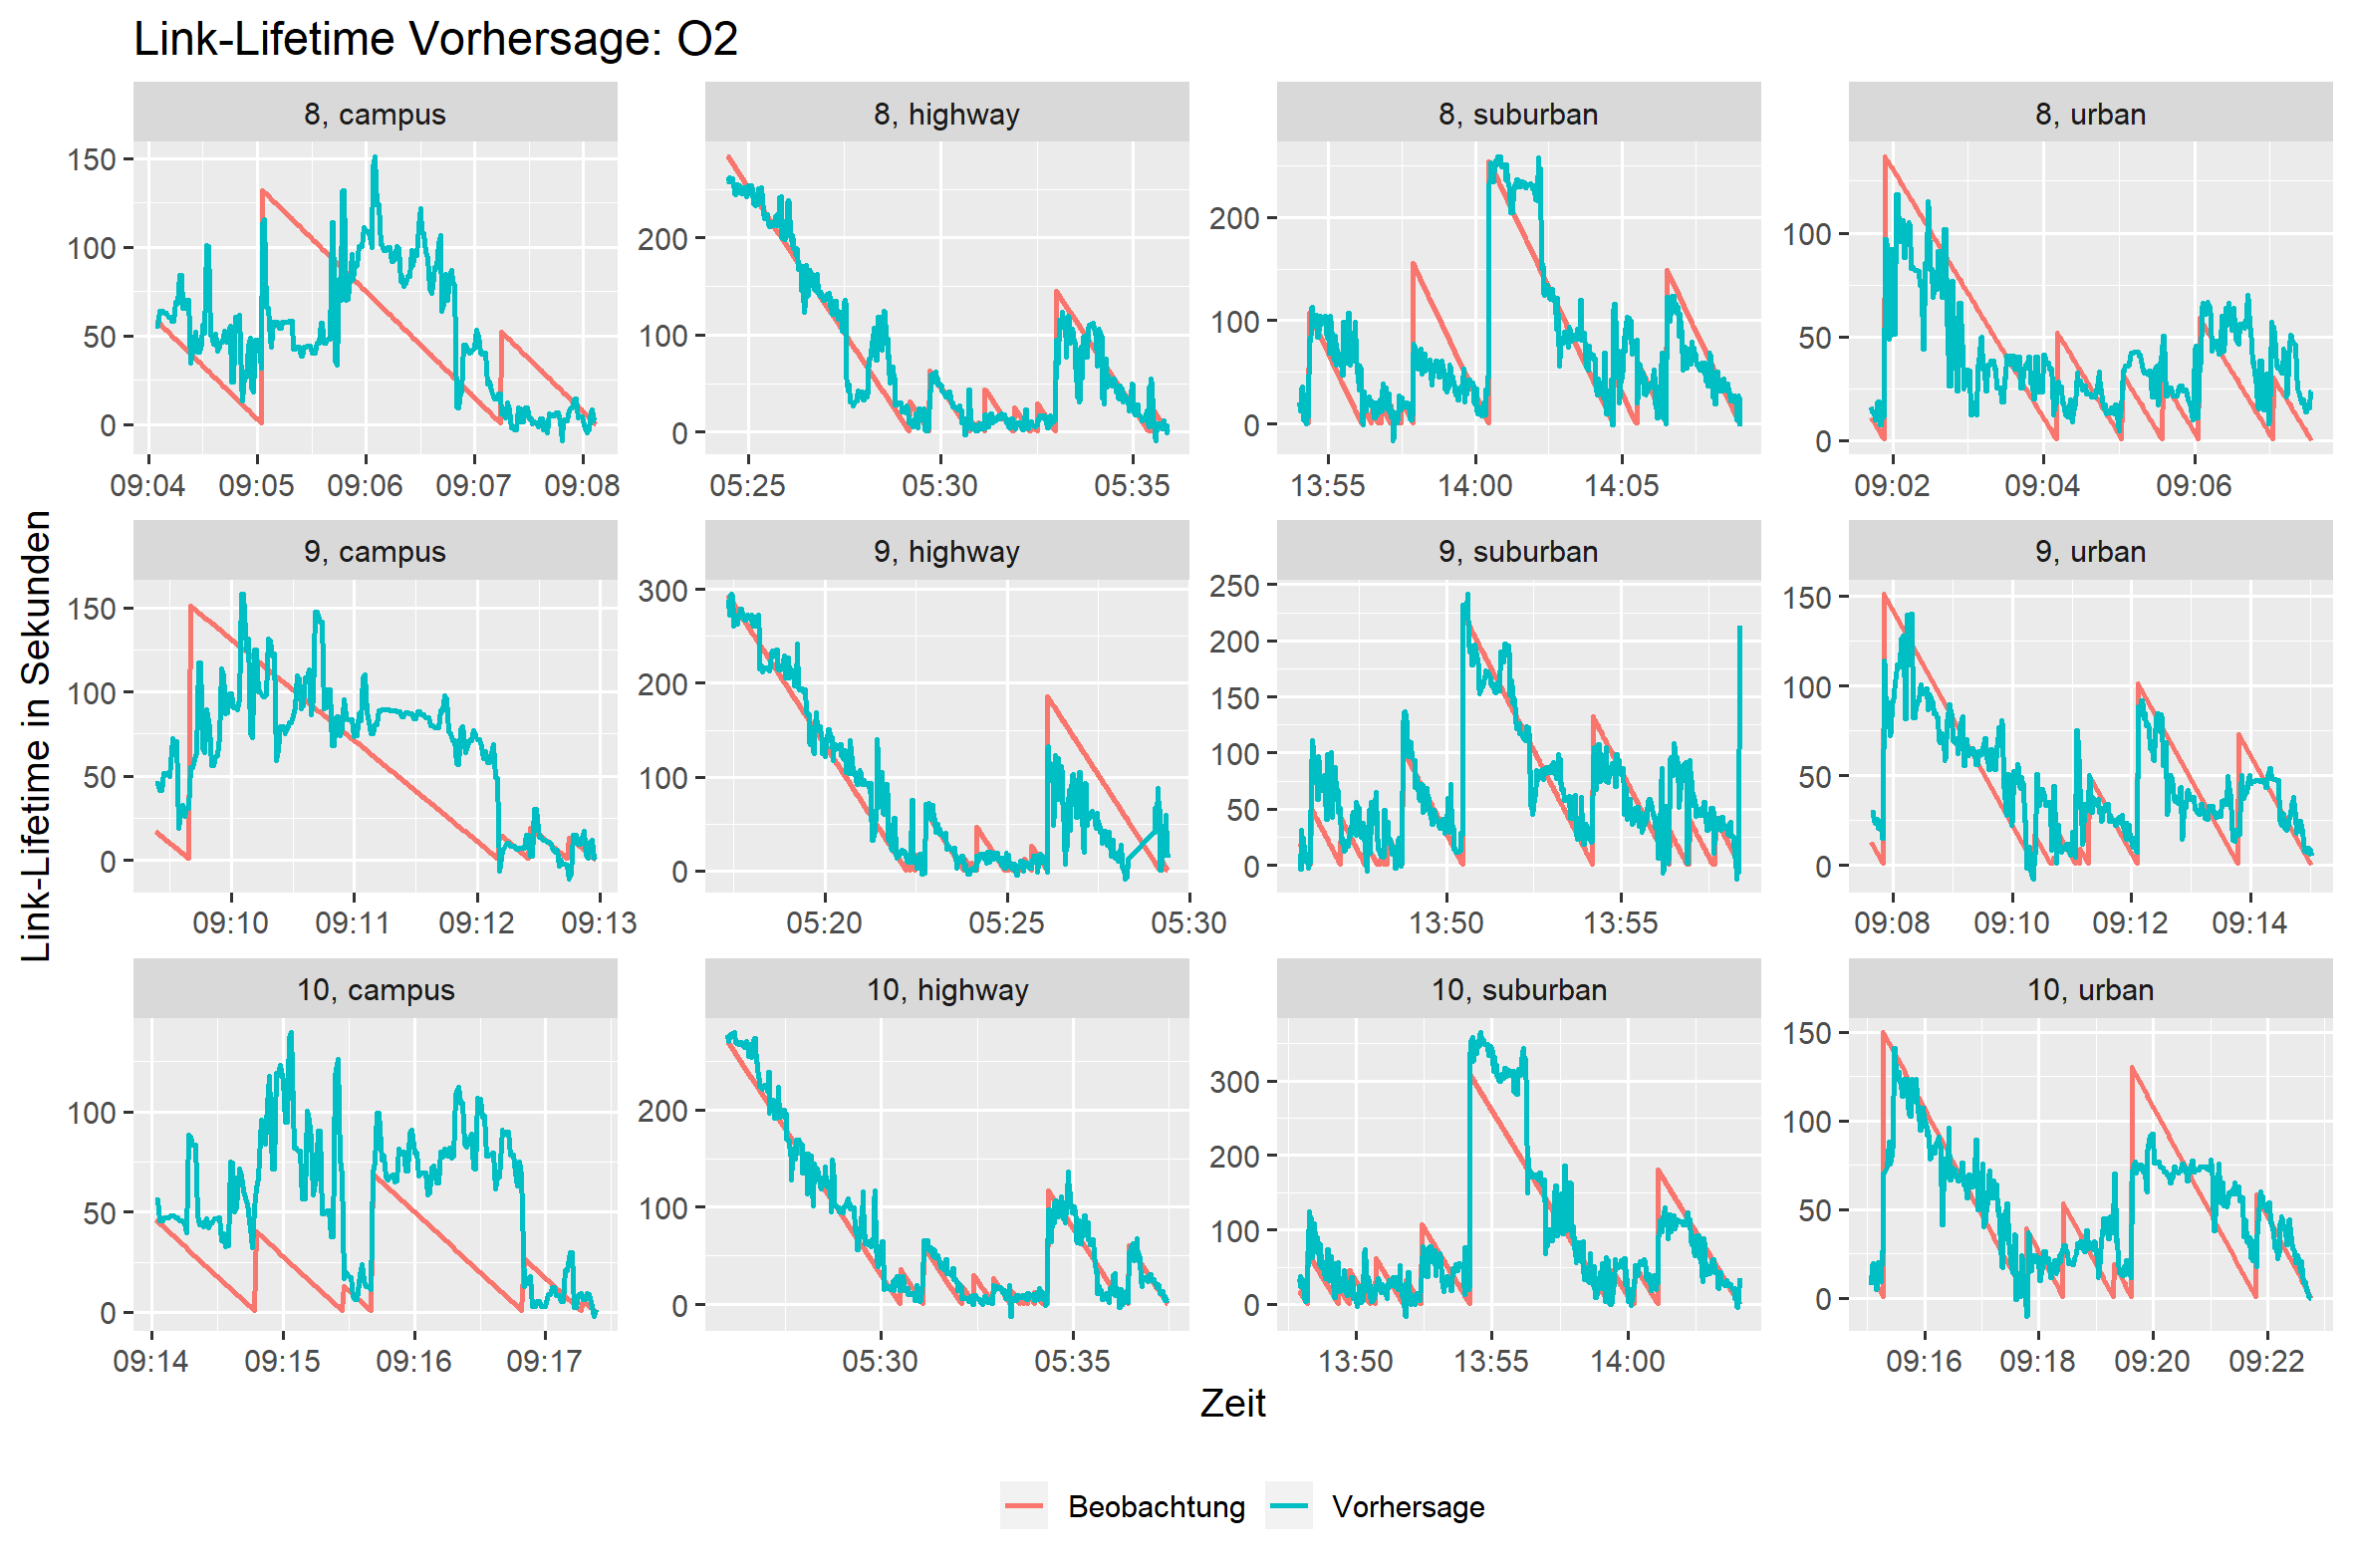
\includegraphics[width=\textwidth]{abbildungen/link_lifetime_o2}
\end{subfigure}
\begin{subfigure}{\textwidth}
    \centering
    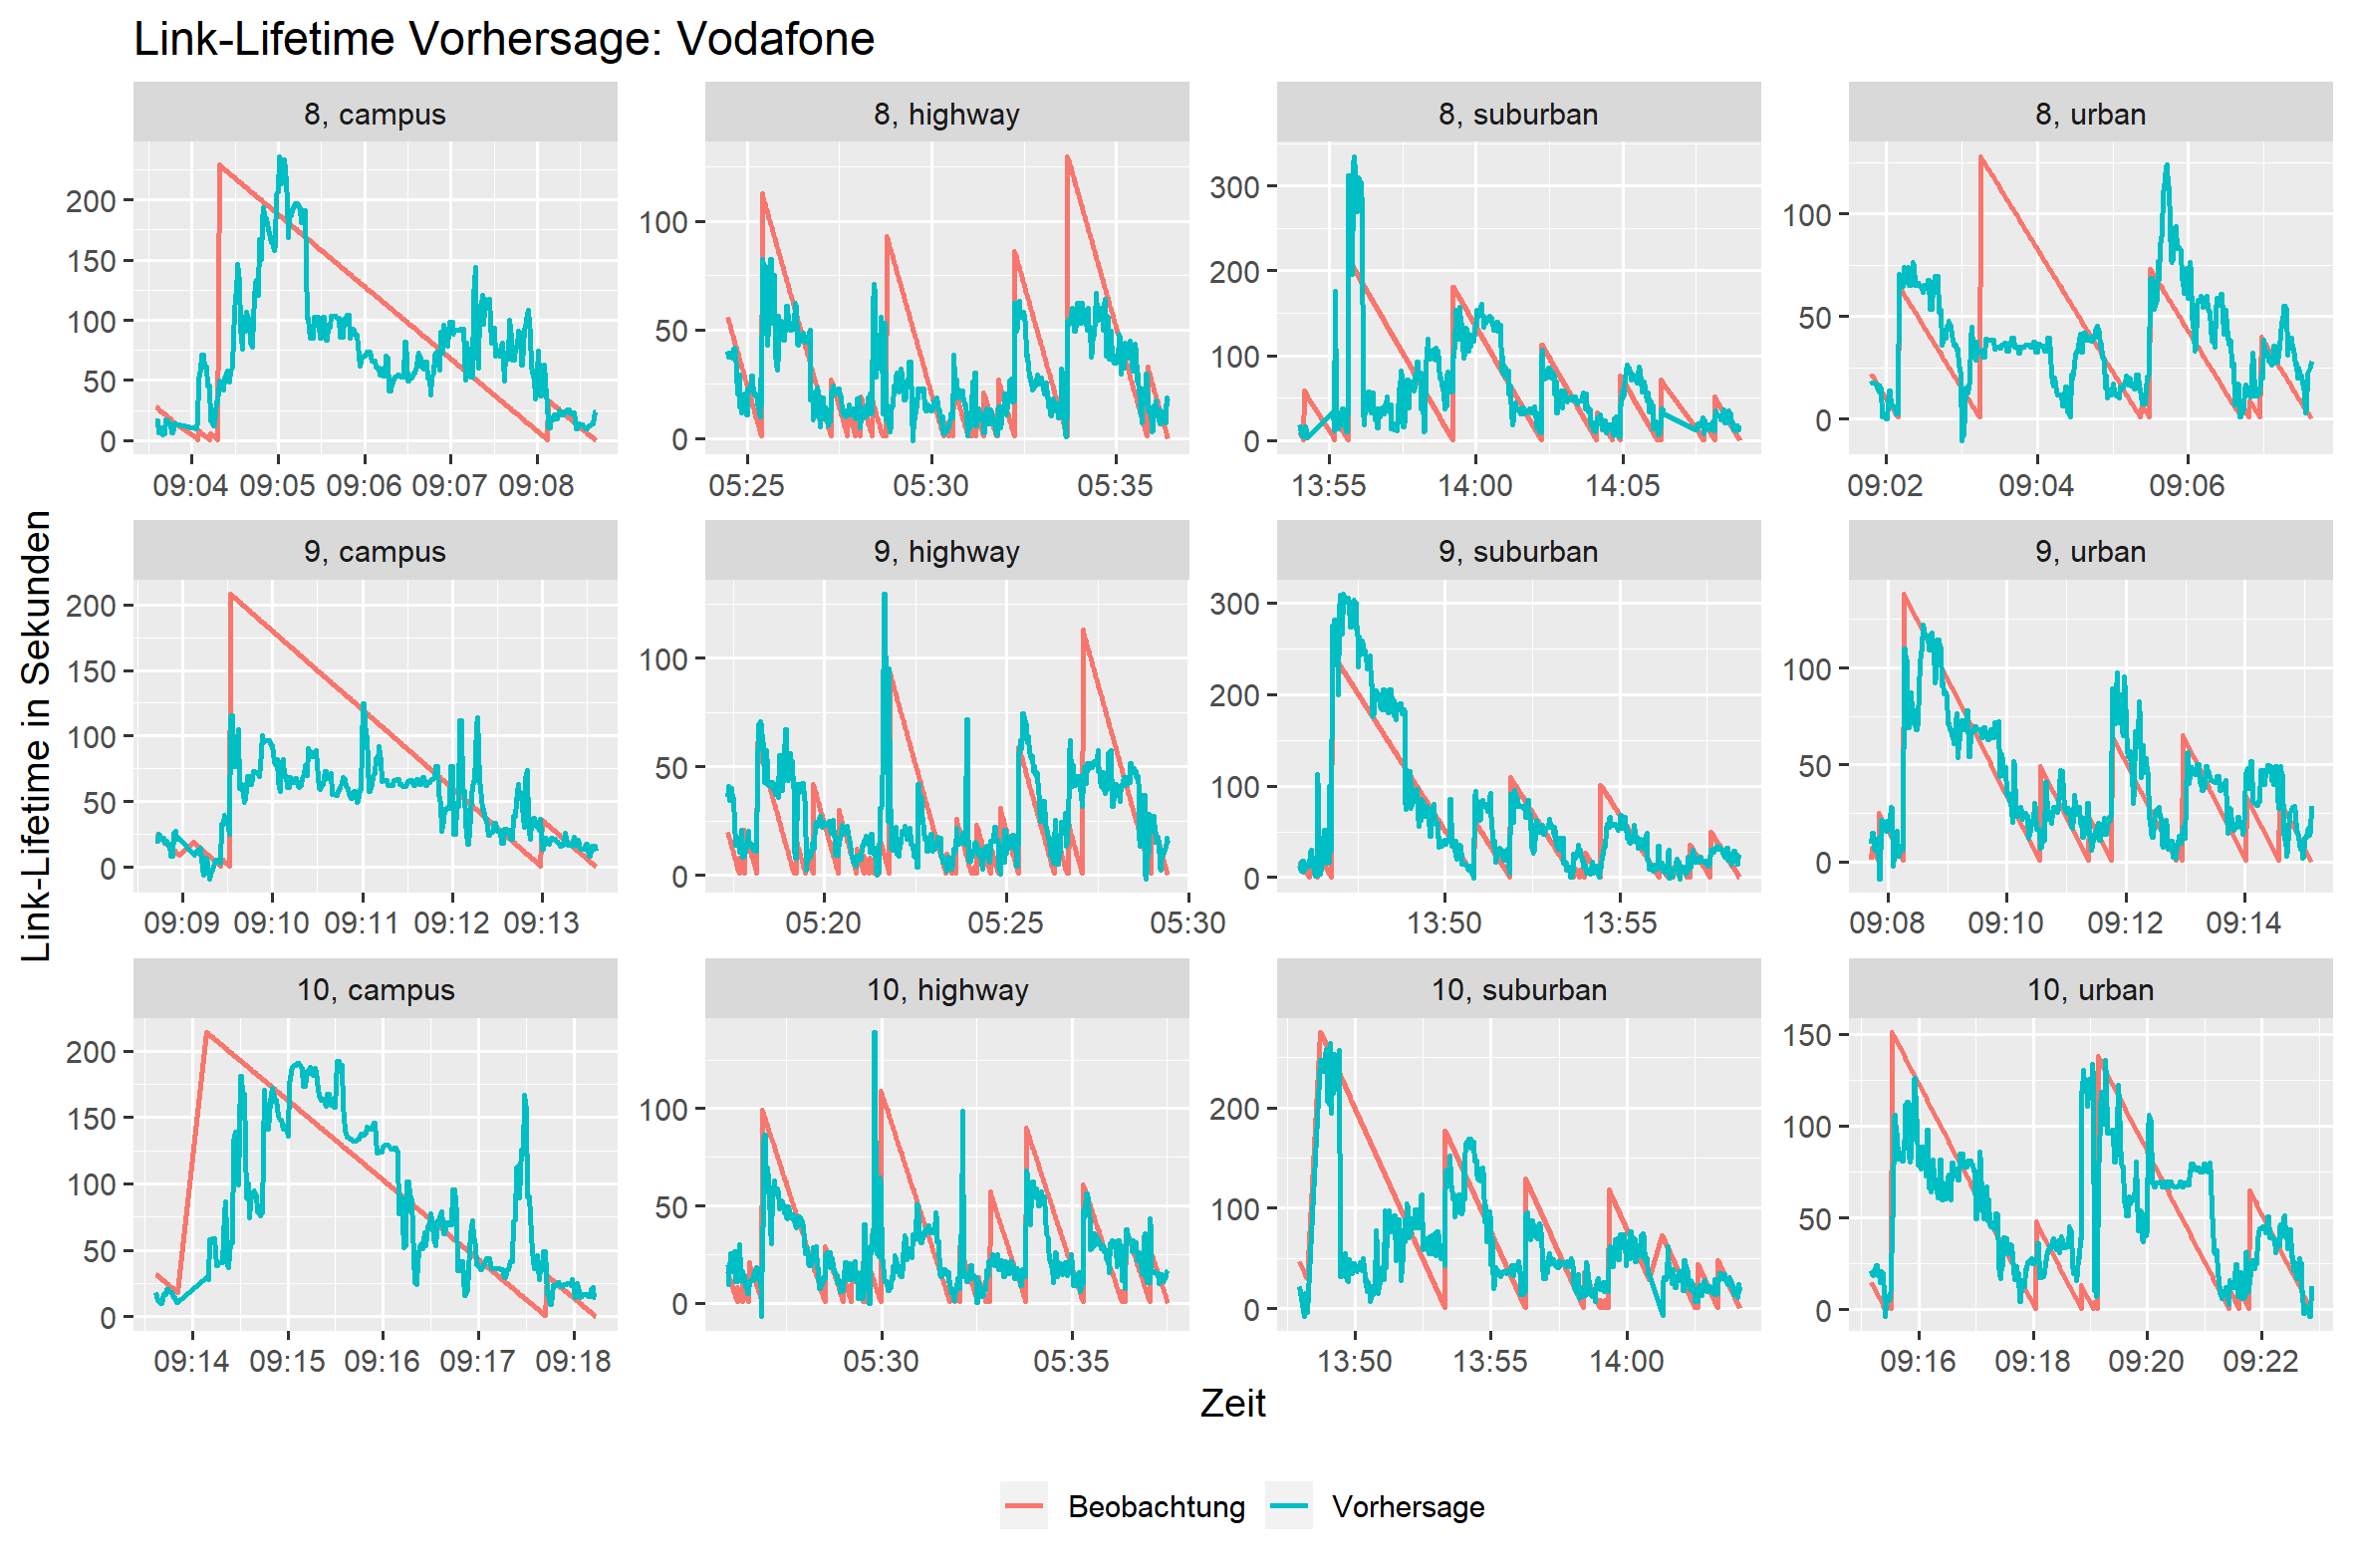
\includegraphics[width=\textwidth]{abbildungen/link_lifetime_vodafone}
\end{subfigure}
\caption{Out-of-Sample Vorhersagen der eNodeB-Verbindungsdauer f\"ur die Anbieter O2 und Vodafone als Zeitreihe.}
\label{fig:link-lifetime-zeitreihe}
\end{figure}

\subsubsection{Relevanz der Kovariablen}

Die Relevanz der Kovariablen wurde hier wie schon bei der Vorhersage der Daten\"ubertragungsraten durch das
Permutation Feature Importance Verfahren ermittelt.
Die resultierenden Werte sind in Abbildung~\ref{fig:feature-importance-link-lifetime} aufgef\"uhrt.

Man erkennt, dass die eNodeB, also die ID des aktuell verbundenen Funkmasts, f\"ur jeden der Provider die relevanteste
Kovariable zu sein scheint. Die Variable Velocity, also die Geschwindigkeit mit der sich das Endger\"at fortbewegt, 
ist ebenfalls sehr relevant. Dies ist auch intuitiv ersichtlich, wenn man sich vorstellt, dass beispielsweise ein schnell
fahrendes Auto \"ofters den Funkmast wechseln muss. Bei den Anbietern O2 und Vodafone scheit zudem das RSRP der Nachbarzelle
noch eine nicht unbedeutende Rolle zu spielen. Dies w\"are dadurch erkl\"arbar, dass eine steigende Signalqualit\"at zu einer
anderen Zelle, welche m\"oglicherweise zu einem anderen Funkmast geh\"ort, ein Indiz f\"ur einen baldigen Funkmastwechsel sein k\"onnte.
Auf der anderen Seite scheinen diese Werte f\"ur den Provider T-Mobile jedoch keine wesentliche Rolle zu spielen.
\begin{figure}
    \centering
    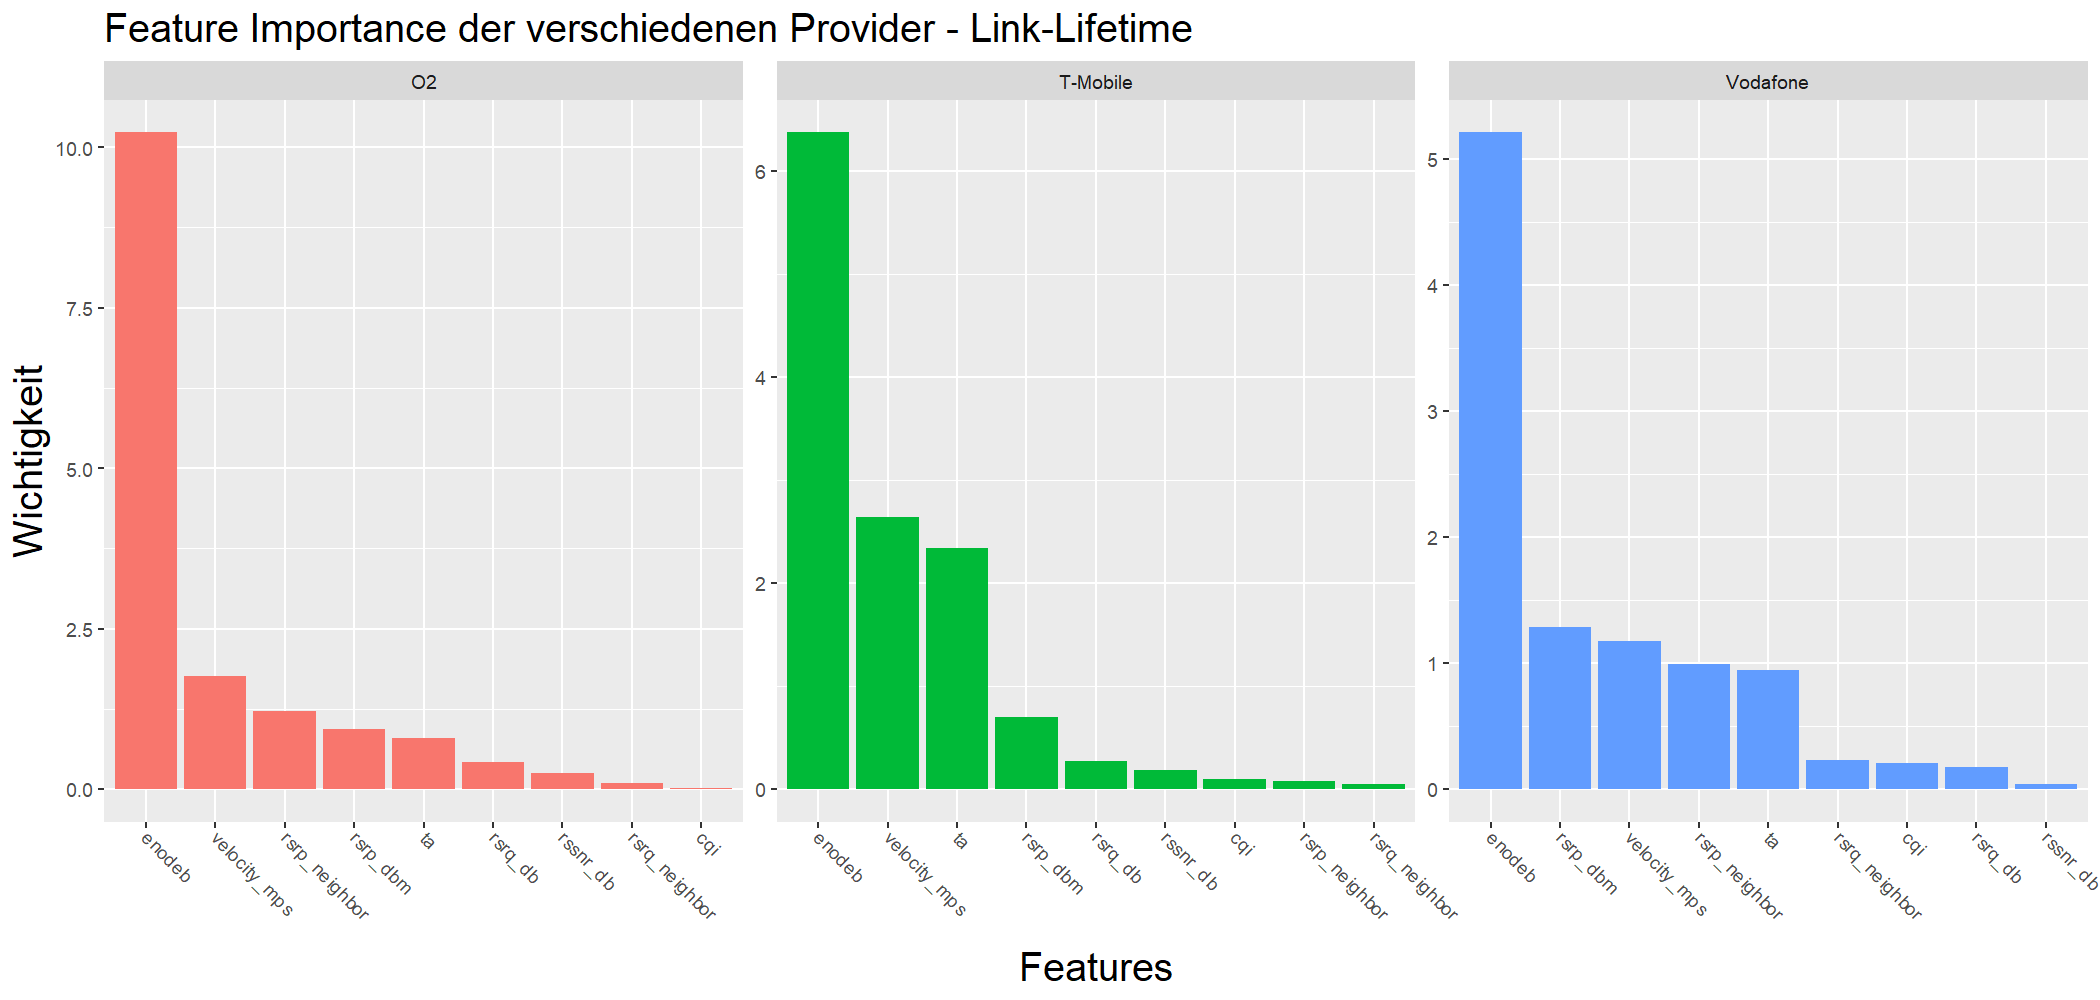
\includegraphics[width=\textwidth]{abbildungen/feature_importance_linklifetime}
    \caption{Feature Importance Link-Lifetime.}
    \label{fig:feature-importance-link-lifetime}
\end{figure}